\documentclass[slovak, master]{diploma}

% Packages (balíky makier)
\usepackage[autostyle=true, czech=quotes]{csquotes} % korektná sadzba úvozoviek, podpora pre balík biblatex
\usepackage[backend=biber, style=iso-numeric, alldates=iso]{biblatex} % bibliografia
\usepackage{dcolumn} % stĺpce tabuľky s číselnými hodnotami
\usepackage{subfig} % makrá pre "podobrázky" a "podtabuľky"
\usepackage[csharp]{diplomalst} % sádzanie
\usepackage{svg}
\usepackage{amsmath}
%\usepackage[python]{diplomalst}
%\usepackage{tcolorbox} % oramovanie

% ------------------------------------------------------

% Definované vlastné metódy, triedy a príslušné farby
% viz bakalarka

% ------------------------------------------------------

% Nový druh tabuľkového stĺpca, v ktorom sú čísla zarovnané podľa desetinnej čiarky
\newcolumntype{d}[1]{D{,}{,}{#1}}

% Odstranenie warningov s underfull vbox
\raggedbottom

% Nastavenie tex color boxu
%\newtcbox{\mybox}[2][black]{outer arc=0pt,  boxsep=0pt, left=0pt, right=0pt, top=0pt, bottom=0pt, boxrule=2pt}

% ------------------------------------------------------

%Zásady pro vypracování
% S umělou inteligencí, která je zodpovědná za rozhodování, se setkáme ve většině počítačových her, ať už jde o hry deskové, plošinové nebo např. tahové. Cílem této diplomové práce je naimplementovat herní prostředí, v němž budou pro rozhodování použity klasické algoritmy jako např. ID3, C4.5, CART (regresní stromy), CHAID (Chi-square, automatic interaction detection), MARS ( (multivariate adaptive regression splines), náhodný les (random forest) a algoritmy jako Deep Q-learning, Double Deep Q-learning, popř. hluboké neuronové sítě a tyto metody porovnat na základě experimentů a následné statistické analýzy. Metody budou porovnány na základě výkonu a úspěšnosti z hlediska řešení daných problémů.

% Zásady pro vypracování:
% 1. Seznamte se s algoritmy jmenovanými výše a způsobem jejich použití v počítačových hrách.
% 2. Navrhněte vlastní netriviální počítačovou hru, kde budou vybrané algoritmy použity pro rozhodování tzv. NPC (non-playing character). Při výběru algoritmů je potřeba, aby byly zastoupeny obě kategorie výše zmíněných algoritmů - tzn. klasické i algoritmy strojového učení. Celkem by mělo být použito aspoň 5 algoritmů, kde aspoň 2 budou patřit do kategorie strojového učení. Ve hře bude implementována postava hráče, který bude proti NPC bojovat.
% 3. Naimplementujte zvolené algoritmy a proveďte jejich srovnání na základě opakovaných experimentů. Během implementace klaďte důraz na efektivitu. Žádný z algoritmů nesmí být proti jinému zvýhodněn. Proveďte statistickou analýzu a s použitím vhodných statistických testů vyhodnoťte kvalitu poskytovaného řešení těchto algoritmů a jejich výkon.
% 4. Výsledky zpracujte v podobě tabulek a grafů a na jejich základě proveďte vyhodnocení testů. Shrňte výhody a nevýhody jednotlivých algoritmů. V závěru uveďte, který algoritmus dosáhl nejlepšího výkonu a který byl při řešení daných úkolů nejúspěšnější.

% ------------------------------------------------------

% Titulná strana
\ThesisAuthor{Bc. Miroslav Kačeriak}
\ThesisSupervisor{prof. Ing. Jan Platoš, Ph.D.}
\CzechThesisTitle{Rozhodování v počítačových hrách - srovnání metod umělé inteligence}
\EnglishThesisTitle{Decision Making in Computer Games - a Comparison of Artificial Intelligence Methods}
\ThesisAssignmentFileName{ThesisSpecification_KAC0067_vsboee22026009.pdf}
\SubmissionYear{2023}

% ------------------------------------------------------

% Abstrakty
\CzechAbstract{TODO}
%TODO - pis po cesky asi

\CzechKeywords{strojové učení, posílené učení, umělá inteligence, rozhodovací stromy, ID3, D4.5, CART, PPO, počítačová hra, Unity engine, C\#, Python}

\EnglishAbstract{TODO}

\EnglishKeywords{machine learning, reinforcement learning, artificial intelligence, decision trees, ID3, D4.5, CART, PPO, computer game, Unity engine, C\#, Python}

% ------------------------------------------------------

% Poďakovanie
\Acknowledgement{Rád by som na tomto mieste poďakoval prof. Ing. Jánovi Platošovi, Ph.D. za pomoc a ochotu prejavenú popri vedení tejto diplomovej práce a mojej priateľke Zdenke za trpezlivosť a prínosné rady, bez ktorých by výsledná práca bola o niečo chudšia.}

% ------------------------------------------------------

% Skratky
\AddAcronym{AI}{Artificial Intelligence}
\AddAcronym{API}{Application Programming Interface}
\AddAcronym{AR}{Augmented Reality}
\AddAcronym{BC}{Behavioral Cloning}
\AddAcronym{CART}{Classification and Regression Tree}
\AddAcronym{CLR}{Common Language Runtime}
\AddAcronym{FOV}{Field Of View}
\AddAcronym{FPS}{Frames Per Second}
\AddAcronym{GAIL}{Generative Adversarial Imitation Learning}
\AddAcronym{GUI}{Graphic User Interface}
\AddAcronym{HW}{Hardvér}
\AddAcronym{ID3}{Iterative Dichotomiser 3}
\AddAcronym{IG}{Information Gain}
\AddAcronym{LINQ}{Language Integrated Query}
\AddAcronym{MA-POCA}{Multi-Agent Posthumous Credit Assignment}
\AddAcronym{MDP}{Markov Decision Process}
\AddAcronym{MS}{Microsoft}
\AddAcronym{NPC}{Non-Playable Character}
\AddAcronym{PPO}{Proximal Policy Optimization}
\AddAcronym{SAC}{Soft Actor-Critic}
\AddAcronym{SQL}{Structured Query Language}
\AddAcronym{TRPO}{Trust Region Policy Optimization}
\AddAcronym{VR}{Virtual Reality}

% ------------------------------------------------------

% Literatúra
\addbibresource{literature.bib}

% ------------------------------------------------------

% Samotný dokument
\begin{document}
\MakeTitlePages

% Zoznam obrázkov
\listoffigures
\clearpage

% Zoznam tabuliek
\listoftables
\clearpage

% Zoznam zdrojakov
\lstlistoflistings
\clearpage

% Chapter 0
\chapter{Úvod}
\label{sec:Introduction}
%TODO
% bla bla uvod
% kladie si za ciel porovnať dva ML pristupy v hre 

% ------------------------------------------------------

% Teória
% Chapter 1
\chapter{Umelá inteligencia v hrách}
\label{sec:AI in games}
%TODO
\chapter{Strojové učenie}
\label{sec:MachineLearningOverview}
Strojové učenie (Machine learning) je vedný obor spadajúci do oblasti umelej inteligencie zaoberajúci sa štúdiom algoritmov a štatistických modelov, na základe ktorých dokáže počítačový systém vykonať určitú úlohu bez nutnosti byť na ňu explicitne naprogramovaný \cite{mahesh2020machine}. Algoritmus strojového učenia na základe vstupných (trénovacích) dát vytvorí model, ktorý môže byť následne využitý na detekciu anomálií v dátach, predikciu či automatizované rozhodovanie. Trénovanie modelu sa nazýva aj proces učenia, od čoho je odvodený aj názov oboru. Strojové učenie je dnes často využívané v rôznych oblastiach ako data mining, image processing, počítačové videnie, spracovanie prirodzeného jazyka, prediktívnu analýzu apod.\cite{zhou2021machine}.
Strojové učenie je možné rozdeliť podľa do troch základných kategórií: %TODO - idealne daj zdroj
\begin{itemize}
  \item \textbf{Supervised learning} -- trieda algoritmov strojového učenia, ktoré sa zaoberajú vytváraním funkcie, ktorá mapuje vstup na výstup na základe príkladu vstupno-výstupných dvojíc. Funkcia je odvodzovaná na základe trénovacích dát, ktoré obsahujú aj premennú, ktorú je chceme klasifikovať či predikovať. Algoritmy sa teda učia vzorce na základe trénovacích dát a tie sa snažia aplikovať na testovacie dáta, ktoré túto premennú neobsahujú, alebo je algoritmu zatajená a je využitá ta určovanie výkonnosti modelu \cite{mahesh2020machine}. Do tejto skupiny spadajú aj rozhodovacie stromy popísané v nasledujúcej sekcií.
  \item \textbf{Unsupervised learning} -- trieda algoritmov strojového učenia, ktoré majú za úlohu analyzovať vstupné dáta a hľadať v nich skryté vzorce bez ľudského pričinenia. Algoritmy hľadajú podobnosti a odlišnosti podskupín dát na základe ktorých je potom možné dáta zhlukovať do rôznych tried, či redukovať počet vlastností odstránením redundantných. Narozdiel od supervised learningu je ma overenie výkonnosti modelu často nutná externá evaluácia doménovým expertom, keďže nie sú prítomné žiadne premenné, s ktorými by sa dali predikované výsledky porovnať. Táto trieda algoritmov je využívaná v prípadoch, kedy nie je možné alebo by bolo veľmi drahé anotovať veľkú dátovú sadu, keď nevieme, koľko skupín sa v dátach nachádza, prípadne, keď potrebujeme získať základnú predstavu o dátach \cite{Unsupervised}. Táto trieda algoritmov nie je vhodná na aplikáciu v umelej inteligencií v hrách a teda v tomto projekte nie je využívaná.
  \item \textbf{Reinforcement learning} -- trieda algoritmov strojového učenia v ktorých sa agent učí vykonávať správne rozhodnutia alebo akcie v prostredí v ktorom operuje. Agent nemá explicitne určené, čo je jeho úlohou a učenie teda prebieha pomocou postupného skúšania rôznych akcií za účelom maximalizácie kumulatívnej odmeny \cite{reinforcementLearning}.
\end{itemize}

\section{Rozhodovacie stromy}
\label{sec:DecisionTreesOverview}
V teórií grafov označuje názov strom súvislý acyklický graf, teda graf, ktorý neobsahuje žiadnu kružnicu. Strom ktorý má jeden vrchol označený ako koreň sa nazýva koreňovým stromom. Zavedením koreňa vzniká orientácia hrán od koreňa cez jeho potomkov až po tzv. listy, čo sú vrcholy, ktoré nemajú žiadnych potomkov \cite{kovavr2012teorie}. 

Rozhodovací strom je teda možné formálne definovať ako koreňový strom, ktorého vnútorné vrcholy reprezentujú test hodnoty určitého atribútu a každý list predstavuje finálne rozhodnutie vykonané po otestovaní všetkých atribútov. Cesty od koreňa k listu predstavujú klasifikačné pravidla \cite{DecTreeTowards}. Príklad rozhodovacieho stromu je možné vidieť na obrázku \ref{pic:decTreeExample}.

\begin{figure}[!htbp]
    \centering
    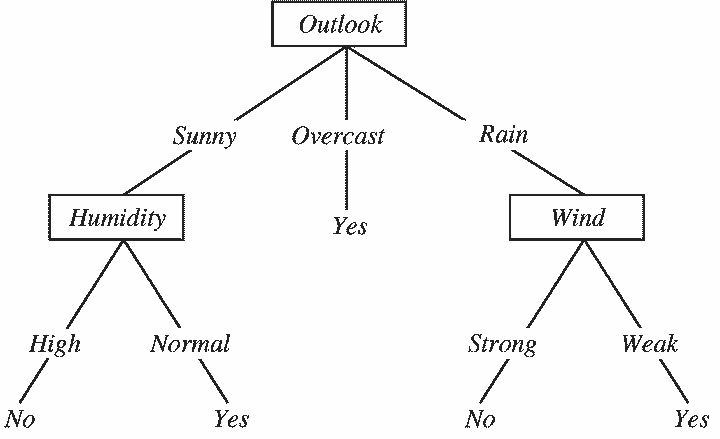
\includegraphics[width=.7\textwidth]{Figures/strom.png}
    \caption{Príklad rozhodovacieho stromu \cite{DecTreeTowards}}
    \label{pic:decTreeExample}
\end{figure}

Rozhodovacie stromy patria do triedy neparametrických supervised learning algoritmov, teda nie sú založené na matematickom modeli definujúcom vzťah medzi vstupom a výstupom. Učia sa teda z dát samotných. Vyznačujú sa vyššou flexibilitou ako parametrické algoritmy ale aj vyššou výpočtovou náročnosťou \cite{paramVSnonparam}. 

Existuje množstvo algoritmov pomocou ktorých je možné zostaviť rozhodovací strom zo vstupných dát. V tomto projekte sú využité algoritmy ID3, D4.5 a CART, ktorých popisu sú venované nasledujúce sekcie. 

\subsection{Algoritmus ID3}
\label{sec:ID3}
ID3, celým názvom Iterative Dichotomiser 3, je klasifikačný algoritmus publikovaný Rossom Quinlanom v roku 1975. ID3 vytvára rozhodovací strom zo vstupnej dátovej sady na základe miery Information Gain (IG). Nakoľko sa výpočet IG do veľkej miery opiera o pojem Entropia, sú obe tieto miery definované v sekcií \ref{sec:ID3miery}. 

Algoritmus na vstupe dostane dátovú sadu vo forme tabuľky, kde jednotlivé riadky je možné predstaviť si ako objekty a stĺpce reprezentujú atribúty týchto objektov. Jeden z týchto atribútov je označený ako cieľový a zostrojený rozhodovací strom bude na základe hodnôt zvyšných atribútov určovať jeho hodnotu. Algoritmus postupuje po iteráciách a v každej iterácií vyberie ne-cieľový atribút s najvyššou hodnotou IG, z ktorého sa stane koreň aktuálneho pod-stromu. Spojením všetkých takto vzniknutých pod-stromov vzniká celý rozhodovací strom \cite{hssina2014comparative}. Pseudokód algoritmu je možné vidieť na obrázku \ref{pic:id3Pseudo}.

\begin{figure}[!htb]
    \centering
    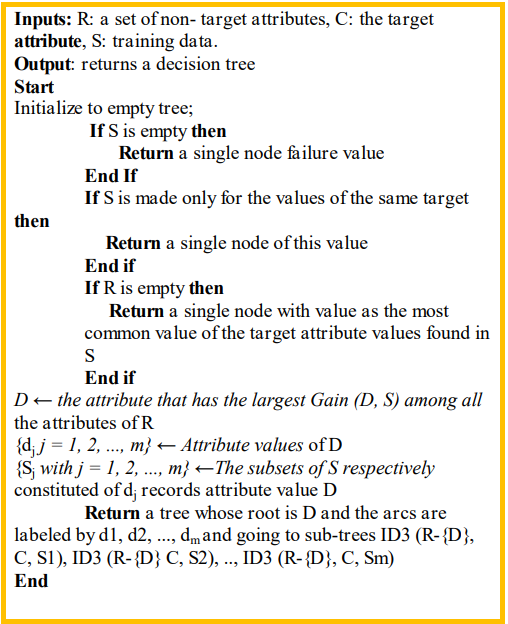
\includegraphics[width=.55\textwidth]{Figures/id3Pseudo.png}
    \caption{Pseudokód algoritmu ID3 \cite{hssina2014comparative}}
    \label{pic:id3Pseudo}
\end{figure}

\subsubsection{Miery využívané algoritmom ID3}
\label{sec:ID3miery}
Entropia je miera v teórií informácií, ktorá vyjadruje neusporiadanosť (neurčitosť) v skupine pozorovaní \cite{EntropyAndGain}. Uvažujme dátovú sadu D s N rôznymi triedami objektov, kde P(\textit{i}) je pravdepodobnosť výberu triedy \textit{i}. Entropia tejto dátovej sady je potom daná vzorcom: 

\[Entropy(D) = -\displaystyle\sum\limits_{i=1}^n P(i) \times \log_2(P(i))\]

Information gain je možné charakterizovať ako mieru toho, koľko informácií o triede \textit{i} poskytuje atribút A, pomocou čoho je neho možné určiť poradie atribútov v rozhodovacom strome \cite{EntropyAndGain}. Gain atribútu A s N rôznymi triedami objektov je teda možné určiť ako:

\[Gain(A) = Entropy(D) - \displaystyle\sum\limits_{j=1}^n P(j) \times E(D_j)\]

kde \textit{j} reprezentuje triedu atribútu A a $D_j$ značí podmnožinu dátovej sady v ktorej všetky objekty spadajú do triedy \textit{j} podľa atribútu A.

\subsection{Algoritmus D4.5}
\label{sec:D45}
Algoritmus D4.5 bol publikovaný v roku 1993 Rossom Quinlanom ako rozšírenie algoritmu ID3 od rovnakého autora. Oba algoritmy sú si koncepčne veľmi podobné. Hlavnou výhodou algoritmu D4.5 oproti algoritmu ID3 je menšia citlivosť na atribúty s veľkým počtom hodnôt a je teda vhodnejší na tento typ vstupnej dátovej sady. Algoritmus D4.5 uprednostňuje pri vytváraní rozhodovacieho stromu atribúty s vyššou hodnotou miery Gain ratio, ktorej výpočet využíva miery Information Gain a Split Info \cite{hssina2014comparative}. Miera IG bola popísaná v predchádzajúcej sekcií v rámci popisu algoritmu ID3, zvyšné miery sú popísané v sekcií \ref{sec:D45miery}.

\subsubsection{Miery využívané algoritmom D4.5}
\label{sec:D45miery}
Mieru Gain Ratio je možné chápať ako normalizovanú hodnotu miery Information Gain \cite{hssina2014comparative}. Jej výpočet je daný vzorcom:

\[GainRatio(A) = \frac{Gain(A)}{SplitInfo(A)}\]

Miera Split Info určuje počet vetiev rozhodovacieho stromu, ktoré by vznikli pri rozdelení podľa daného atribútu. Je daná vzorcom:

\[SplitInfo(A) = - \displaystyle\sum\limits_{j=1}^n P(j) \times \log_2(P(j))\]

\subsection{Algoritmus CART}
\label{sec:CART}
Algoritmus CART, celým názvom Classification and Regression Tree podobne ako algoritmy ID3 a D4.5 vytvára rozhodovací strom zo vstupnej dátovej sady. Ako napovedá jeho názov je možné ho použiť na úlohy vyžadujúce klasifikáciu aj regresiu. Výstupom tohto algoritmu je vždy binárny rozhodovací strom, teda každý vrchol, ktorý nie je listom má práve dvoch potomkov \cite{CART}. Princíp fungovania algoritmu je opäť veľmi podobný algoritmom ID3 a D4.5. Metrikou použitou pre posúdenie kvality rozdelenia je Gini Index.

Gini index vyjadruje pravdepodobnosť, že náhodne vybraný objekt bude nesprávne klasifikovaný podľa distribúcie tried v dátovej sade. Hodnota Gini indexu sa pohybuje na škále 0--1, kde 0 značí, že všetky objekty patria do jednej triedy alebo v dátovej sade existuje iba jedna trieda, 1 značí, že objekty sú náhodne rozložené medzi triedami a hodnota 0,5 značí rovnomerné rozloženie objektov medzi triedami \cite{Gini}. Výpočet je daný vzorcom:

\[Gini(A) = 1 - \displaystyle\sum\limits_{i=1}^n P(i)^2\]

\section{Reinforcement learning}
\label{sec:ReinfoOverview}
Ako už bolo spomenuté na začiatku tejto kapitoly, algoritmy strojového učenia spadajúce do triedy reinforcement learningu sa vyznačujú tým, že pracujú s Agentom, ktorý je vložený do určitého prostredia a učenie prebieha na základe spätnej väzby. Agent nemá explicitne určené, čo je jeho cieľom. 

Formálne je možné proces popísať na základe MDP, ktorý umožňuje matematicky modelovať rozhodovací proces agenta v dynamickom prostredí. Tento model pracuje s pojmami agent, stav, akcia, odmena a policy. Po vykonaní určitej akcie \textit{A} v danom prostredí sa Agent dostane do stavu \textit{S}. Agent dostáva spätnú väzbu vo forme odmeny \textit{R} na základe akcií, ktoré vykoná a stavu, do ktorého sa dostane. Policy určuje optimálnu akciu agenta na základe aktuálneho stavu s cieľom maximalizovať odmenu \cite{Markov}. Zápornú hodnotu odmeny je možné chápať ako trest. Opakovaním daného postupu potom agent upravuje svoj rozhodovací proces. Tento postup je znázornený na obrázku \ref{pic:reinfoPic}.
  
\begin{figure}[!htbp]
    \centering
    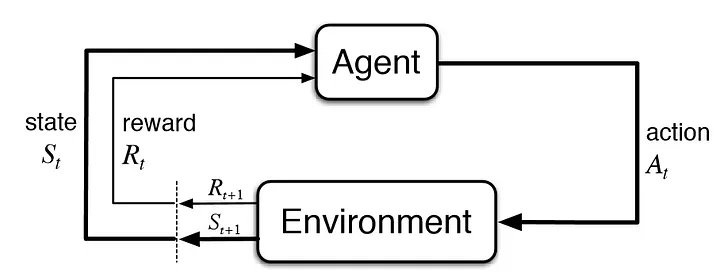
\includegraphics[width=.8\textwidth]{Figures/reinfoGraph.png}
    \caption{Princíp reinforcement learningu \cite{reinfoGraph}}
    \label{pic:reinfoPic}
\end{figure}

Algoritmy reinforcement learningu sú vhodné na aplikáciu v robotike, pri spracovaní prirodzeného jazyka, v samo-riadiacich autách apod. Reinforcement learning by mohol do budúcna priniesť zaujímavé výsledky aj na poli AI v počítačových hrách. V minulosti vznikli projekty v rámci ktorých dokázali agenti s využitím algoritmov reinforcement learningu hrať hry ako Go, StartCraft II či Dota 2 \cite{app13042443}. Na ich využitie vo väčšom komerčnom projekte sa však stále ešte čaká. Časť tejto práce sa venuje práve problematike ich nasadenia v 3D hernom prostredí.

V tomto projekte bol ako zástupca triedy algoritmov reinforcement learningu zvolený algoritmus PPO, teda Proximal Policy Optimization, ktorý je bližšie popísaný v nasledujúcej sekcií.

%TODO - Pridaj nad aj pod zmienky o pripadnom dalsom algoritme ak sa podari

\subsection{Proximal Policy Optimization}
\label{sec:PPO}
Proximal Policy Optimization (PPO) je algoritmus reinforcement learningu, ktorý bol publikovaný v roku 2017 vedcami zo spoločnosti OpenAI. Hlavnými výhodami oproti jeho predchodcovi TRPO (Trust Region Policy Optimization) publikovanom v roku 2015 sú jednoduchšia implementácia, vyššia obecnosť a nižší nutný počet trénovacích vzoriek na naučenie cieľovej funkcie podľa empirického pozorovania \cite{PPOPaper}.

Pri supervised learningu je možné relatívne jednoducho implementovať cost funkciu a pomocou metódy gradient descent dosiahnuť dobrých výsledkov bez nutnosti náročného ladenia hyper-parametrov. Výsledky dosiahnuté pomocou algoritmov reinforcement learningu sú však veľmi citlivé na zmeny týchto parametrov. Algoritmus PPO sa snaží hľadať rovnováhu medzi zložitosťou implementácie, nutným počtom trénovacích vzoriek a práve ladením hyper-parametrov \cite{PPOPaper}.

Algoritmus PPO využíva tzv. policy gradient method \cite{PPOPaper}, čo znamená, že narozdiel napríklad od algoritmov Q-learningu sa agent neučí z uložených predchádzajúcich pokusov ale priamo aktuálne vykonaných akciách v prostredí. Nevýhodou tohto typu algoritmov býva menšia efektivita využitia trénovacích vzoriek, nakoľko vzorky nie sú využité pri učení opakovane, a teda vyššie nároky na ich počet. Ako už však bolo spomenuté. túto nevýhodu sa PPO snaží minimalizovať.  

Algoritmus sa v každom kroku snaží minimalizovať cost funkciu pomocou malých odchýlok od predchádzajúcej policy. Maximálna veľkosť odchýlky je zabezpečená pomocou funkcie clip() v objective funkcií a dá sa ladiť pomocou hyper-parametru \(\varepsilon\) \cite{PPOPaper}. Objective funkcia, ktorá sa typicky nevyskytuje v iných algoritmoch, je nasledovná:

\[L^{CLIP}(\theta) = \hat{E}_t [min(r_t(\theta))\hat{A}_t, clip(r_t(\theta), 1 - \varepsilon, 1 + \varepsilon)\hat{A}_t]\]

kde:
\begin{itemize}
  \item \(\theta\) je parameter policy
  \item \(\hat{E}_t\) označuje empirické očakávanie v priebehu časového kroku
  \item \(r_t\) je pomer pravdepodobnosti podľa novej a starej policy
  \item \(\hat{A}_t\) je odhad výhody v čase \textit{t}
  \item \(\varepsilon\) je hyper-parameter, obecne nadobúda hodnotu v rozsahu 0,1--0,2
\end{itemize}

Objective funkcia sa teda snaží optimalizovať očakávanie v priebehu časového kroku \(\hat{E}_t\). Hodnota \(\hat{E}_t\) je daná menšou z hodnôt \(r_t(\theta))\hat{A}_t\), čo je normálna policy, a jej variantou obmedzenou hyper-parametrom \(\varepsilon\). Toto obmedzenie zabraňuje veľkým zmenám od predchádzajúcej policy. Priebeh funkcie v závislosti toho, či je odhad výhody kladný alebo záporný je možné vidieť na obrázku \ref{pic:clipping}.

\begin{figure}[!htbp]
    \centering
    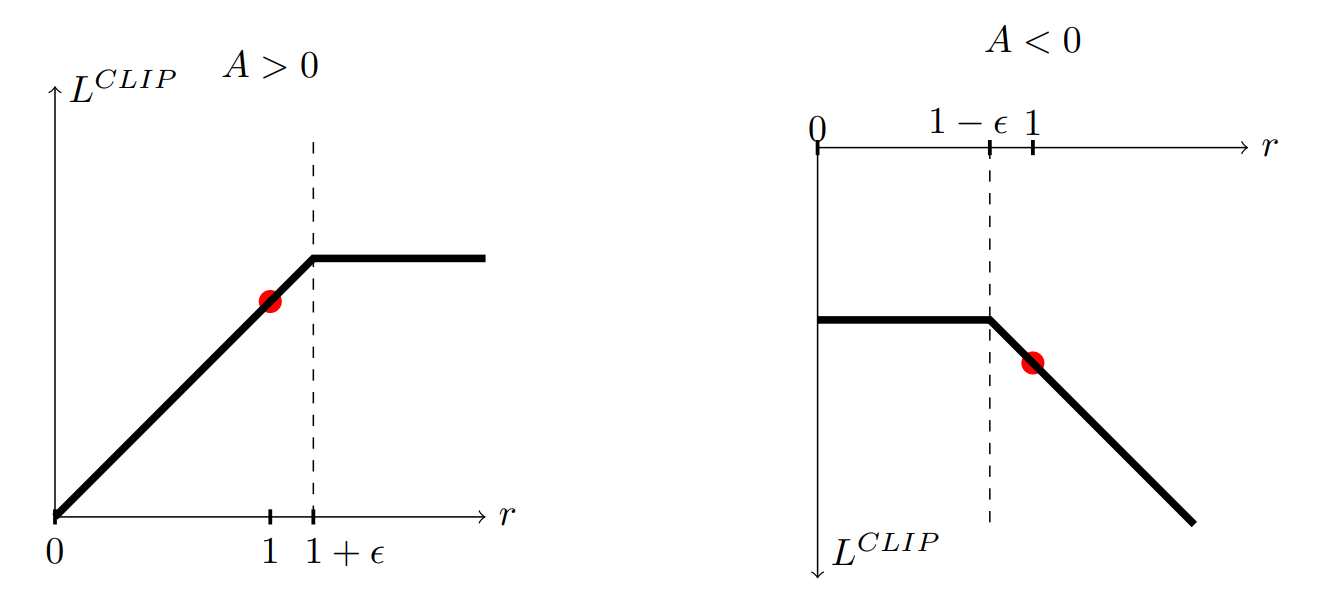
\includegraphics[width=.7\textwidth]{Figures/clip.png}
    \caption{Priebeh objective funkcie pre kladný a záporný odhad výhody \cite{PPOPaper}}
    \label{pic:clipping}
\end{figure}

% ------------------------------------------------------

% Vypracovanie
% Chapter 3
\chapter{Použité technológie}
\label{sec:Tech}
V tejto kapitole sú v stručnosti popísané najdôležitejšie technológie využívané pri tvorbe tohto projektu. Čast textu je zameraná aj na popis motivácie, ktorá viedla k využitiu daných technológií, ich výhody, nevýhody, prípadne zvažované alternatívy z hľadiska vhodnosti pre projekt celkovo, či jeho dielčie časti.

\section{Unity Engine}
\label{sec:Unity}
Unity je herný engine určený k tvorbe 2D a 3D interaktívneho obsahu renderovaného v reálnom čase vyvíjaný spoločnosťou Unity Technologies od roku 2005 \cite{Unity}. Engine je vytvorený v programovacom jazyku C++ ale vývoj obsahu prebieha v jazyku C\# či pomocou vizuálneho skriptovacieho nástroja Bolt vo forme rozšírenia od spoločnosti Unity Technologies. V posledných rokoch sa vývoj enginu Unity sústredí primárne na menšie hry a mobilný trh s dôrazom na monetizáciu mobilných hier pomocou mikro-transakcií a analytické nástroje pre vývojárov. Engine samotný však umožňuje tvorbu rôzneho druhu obsahu pre širokú škálu platforiem od herných konzolí cez desktopové operačné systémy až po VR, MS HoloLens, AndroidTV či web vo forme WebGL \cite{UnityMultiplatform}. Engine Unity je možné využívať zdarma v rámci štúdia či pri malých projektoch, ktorých predaje nepresahujú čiastku \$100K za posledných 12 mesiacov \cite{UnityPersonal}.

Engine Unity bol pri tvorbe tohto projektu zvolený z dôvodu predchádzajúcich skúseností, možnosti tvorby v programovacom jazyku C\#, množstvu dostupných materiálov a kvalite dokumentácie, ktorému sa konkurencia hlavne v podobe enginu Unreal nemôže rovnať. Taktiež umožňuje rýchlejšiu tvorbu a prototypovanie ako väčšina konkurenčných nástrojov a rozsah projektu si nevyžadoval špeciálne nástroje a technológie obsiahnuté napríklad v už spomínanom konkurenčnom engine Unreal. Zároveň sa pomocou projektov ako ML-Agents či Perception čoraz viac stáva vyhľadávanou platformou na poli výskumu a tvorby v oblasti strojového učenia.

\section{Programovacie jazyky}
\label{sec:langs}
V tomto projekte sú využité dva programovacie jazyky. Hlavným jazykom je jazyk C\#, ktorý je využitý pri ovládaní hráčskej postavy, kamery, agentov, na detekciu interakcie s objektami atď. Druhým využitým jazykom je Python. V tomto jazyku sú naprogramované algoritmy ID4, C4.5 a CART popísané v sekcií \ref{sec:DecisionTreesOverview}. Toto rozdelenie je využité z dvoch dôvodov. Prvým je lepšia podpora knižníc v jazyku Python na spracovanie dátových rámcov. Druhým dôvodom bola snaha oddeliť spracovanie vstupných dát pre algoritmy od hlavnej aplikácie, aby nemusela opakovane prejsť buildom pri úprave či pridaní nového algoritmu. Človek, ktorý dizajnuje/upravuje chovanie NPC teda nemusí mať prístup k projektu ale iba nahradí príslušné textové dokumenty v zložke s buildom hry. Nasledujúce sekcie sú venované krátkemu popisu týchto programovacích jazykov.

\subsection{Programovací jazyk C\#}
\label{sec:langsCShartp}
C\# je univerzálny vysoko-úrovňový multi-paradigmatický staticky typovaný programovací jazyk predstavený v roku 2000 spoločnosťou Microsoft. Od svojho predstavenia je jazyk C\# neustále vyvíjaný a obohacovaný o nové vlastnosti. Primárnou paradigmou C\# je objektovo orientované programovanie, poskytuje však množstvo vlastností funkcionálnych jazykov ako LISP či Haskell. Základná syntax C\# je podobná jazykom C, C++ a Java, tá je však obohatená o unikátne prvky ako LINQ, ktoré by sa dali pripodobniť skôr jazyku SQL. C\# má integrovanú automatickú správu pamäte vykonávanú tzv. Garbage Collectorom \cite{DotNetBook}. Výhodou tejto správy je, že nekladie nároky na vývojára, aby pamäť ručne uvoľňoval, robí to však z jazyka C\# nie úplne najvhodnejšiu voľbu na určité výkonovo-orientované aplikácie, ktorými sú aj moderné vysoko-rozpočtové herné tituly. Toto je však možné sčasti obísť metódami ako object pooling apod.

Spolu s jazykom C\# je nutné spomenúť aj .NET ekosystém, vyvíjaný priamo firmou MS, ktorý poskytuje runtime prostredie CLR a širokú škálu knižníc a možností umožňujúcich pohodlné nasadenie C\# v rôznych webových, desktopových či cloudových aplikáciách \cite{DotNetBook}.

Engine Unity využíva jazyk C\# vo verzií 9.0 a kompilátor Roslyn. Nie všetky vlastnosti jazyka C\# 9.0, ako napríklad kovariantné návratové typy sú však v Unity dostupné \cite{compiler}. To isté platí aj o knižniciach .NET ekosystému. Spoločnosť Unity odporúča využívať špecifikáciu .NET Standard, kde je zaručená najväčšia kompatibilita s rôznymi platformami. Podporovaná verzia .NET Standard potom závisí od verzie samotného enginu \cite{netUnity}. 

Jedným z posledných aspektov jazyka C\#, ktorý sa silne neodporúča využívať sú operátory ?? a ? u potomkov triedy UnityEngine.Object, nakoľko tieto operátory nie je možné overridnuť narozdieľ od operátorov == a !=. Dôvodom je, že po pokuse odstrániť tieto objekty z pamäte, sa síce odstránia v natívnom C++ kóde ale v jazyku C\# sa o to musí postarať Garbage Collector. V čase medzi odstránením objektu z natívneho C++ kódu a manažovaného C\# kódu teda operátory ??, ? a ==, != vracajú nekonzistentné výsledky \cite{netUnity}.

\subsection{Programovací jazyk Python}
\label{sec:langsPython}
Python je podobne ako jazyk C\# vysoko-úrovňový multi-paradigmatický jazyk, ktorý je však dynamicky typovaný a čisto interpretovaný. Predstavený bol už v roku 1991, dodnes sa však teší veľkej popularite a podlieha kontinuálnemu vývoju. V dobe písania tejto práce má najaktuálnejšia verzia označenie 3.11. 

Vďaka strmej učebnej krivke a úspornej syntaxi je často využívaný vo výučbe programovania či prototypovaní. Okrem toho je ale veľmi využívaný na poli strojového učenia a dátovej analýzy, vo webovom vývoji či automatizácií rôznych úkonov. Obsahuje širokú škálu knižníc ako pandas, numpy, matplotlib či frameworkov ako Django, Flask apod., ktoré sú vytvárané komunitou či rôznymi spoločnosťami a robia z jazyka python tak obľúbený nástroj. Nevýhodou jazyka je jeho výkon. Nakoľko interpretácia python kódu je relatívne pomalá operácia, nemôže z tohto hľadiska dobre konkurovať iným kompilovaným jazykom. Túto nevýhodu dokáže sčasti prekonať jeho dobrá integrácia s jazykmi C a C++, čo umožňuje vytvárať knižnice priamo v týchto jazykoch a tým optimalizovať kritické časti kódu či náročné matematické operácie \cite{pajton}.

\section{Nástroj ML-Agents}
\label{sec:ML-Agents}
ML-Agents \cite{mlagents} je open-source projekt, ktorý umožňuje využiť prostredie vytvorené v engine Unity na tréning agentov pomocou algoritmov reinforcement learningu ako napríklad už spomínaný algoritmus PPO ale aj SAC, MA-POCA a ďalších. Okrem reinforcement learningu obsahuje ML-Agents aj podporu pre algoritmy imitation learningu ako BC a GAIL, neuro-evolúciu apod. ML-Agents poskytuje implementáciu týchto algoritmov založenú na python frameworku PyTorch spolu s klient-server komunikáciou medzi enginom Unity a týmito algoritmami v pythone. Taktiež ponúka možnosť importu vytrénovaných modelov naspäť do enginu, kde je možné na základe nich nechať agentov vykonávať rozhodnutia, či dotrénovať určitý model na základe nových situácií. Týchto agentov je možné trénovať či testovať v kontexte 2D, 3D či VR/AR hier a vedeckých simulácií. Okrem ovládania NPC je nástroj ML-Agents možné využiť aj v oblastiach ako automatizované testovanie apod.

Nástroj ML-Agents poskytuje množstvo komponentov na strane Unity napísaných v jazyku C\#, ktoré je možné využiť či ďalej rozšíriť, aby vyhovovali potrebám takmer všetkých scenárov. Okrem toho však ML-Agents poskytuje Python API na tvorbu či úpravu trénovacích algoritmov, u ktorých je samozrejme možné rôzne ladiť hyper-parametre pomocou štruktúrovaných textových súborov. Vizualizácia učebnej krivky agentov realizovaná pomocou nástroja TensorBoard.

ML-Agents je neustále vyvíjaný a jeho posledná stabilná verzia 20 vyšla v novembri 2022. Medzi najväčšie limitácie patrí podpora buildu iba pre platformy Windows, Mac a Linux. Tá je však obmedzená iba na scripting backend Mono a teda nie je teda možné využiť IL2CPP \cite{mlagentsGit}. Oba tieto problémy sa však týkajú primárne väčších komerčných projektov a v tomto prípade neboli prekážkou. 

Hlavným dôvodom pre výber tohto nástroja bola jeho otvorenosť a priama podpora enginu Unity z hľadiska poskytovaných komponentov, medziprocesovej komunikácie a následného nasadenia modelu. V prípade zvolenia iného riešenia či vlastnej implementácie by všetky tieto aspekty museli byť vytvorené na mieru a bez kontinuálnej podpory, ktorú nástroju ML-Agents poskytuje komunity, by takéto riešenie rýchlo prestalo byť funkčné v novších verziách enginu Unity.

\begin{figure}[!htbp]
    \centering
    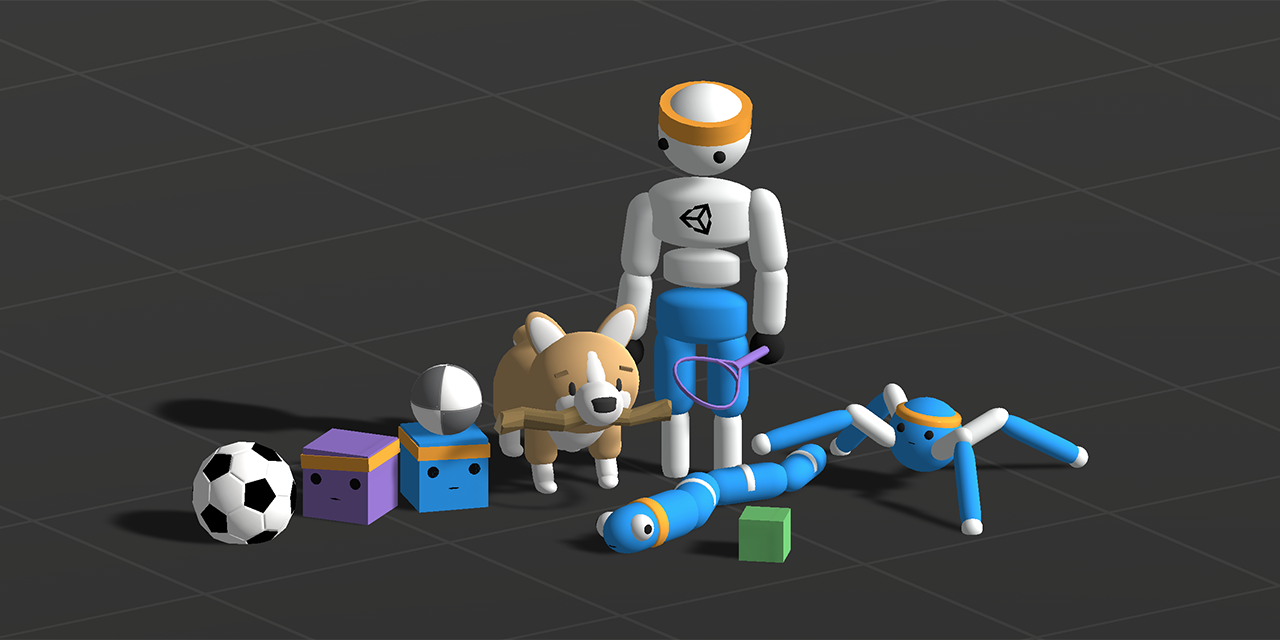
\includegraphics[width=1\textwidth]{Figures/mlagents.png}
    \caption{Titulný obrázok ML-Agents \cite{mlagentsWeb}}
    \label{pic:mlagetnsLogo}
\end{figure}

\subsection{Inštalácia prvotné nastavenie}
\label{sec:MLAgentsInstall}
Pre využitie nástroja ML-Agents je nutné mať nainštalovaný program Python. Podporovaná verzia jazyka sa líši v závislosti od konkrétneho releasu ML-Agents. V tomto projekte bol využitý ML-Agents v release 19 a Python vo verzií 3.9.13. Nakoľko je nástroj ML-Agents citlivý na verzie rôznych knižníc bolo pre účel tohto projektu vytvorené uzavreté prostredie pomocou open-source distribúcie Anaconda. Tento krok však nie je povinný. Následne je nutné stiahnuť konkrétny release korešpondujúci s verziou enginu Unity z platformy GitHub, rozbaliť archív a v príkazovom riadku sa navigovať do rozbalenej zložky.

Následne je nutné pomocou manažéra python balíkov pip spustiť nasledujúce príkazy:
\begin{itemize}
  \item pip3 install torch -f https://download.pytorch.org/whl/torch\_stable.html
  \item pip3 install -e ./ml-agents-envs
  \item pip3 install -e ./ml-agents
\end{itemize}

Prvý spomenutý príkaz sa pokúsi stiahnuť poslednú stabilnú distribúciu knižnice PyTorch. Tento krok však môže zlyhať z rôznych problémov s kompatibilitou HW a v takomto prípade je nutné knižnicu stiahnuť ručne pomocou konfigurátoru na stránke PyTorch alebo v archíve distribúcií. Nakoľko sa verzie knižnice líšia aj v závislosti od modelovej rady procesoru nie je možné jednoducho vytvorený Anaconda environment jednoducho distribuovať medzi zariadeniami. Zvyšné dva príkazy nainštalujú knižnice ml-agents-envs a ml-agents z lokálneho úložiska. Pri inštalácií záleží na poradí.

Následne je nutné vytvoriť projekt v engine Unity alebo použiť už existujúci. Podporované verzie pre konkrétny release ML-Agents je opäť možné nájsť v dokumentácií. Tento projekt je postavený na verzií 2022.2.0b12. Do vytvoreného projektu je nutné pridať C\# rozšírenie ML-Agents. 

Postup je nasledovný: 
\begin{itemize}
  \item V ponuke \textit{Window > Package Manager} kliknúť na ikonu + a z drop-down menu vybrať vybrať voľbu \textit{Add Package from disk}
  \item V následnom dialógu vybrať súbor \textit{package.json} v zložke \textit{com.unity.ml-agents}, ktorá sa nachádza medzi súbormi stiahnutými z GitHubu
\end{itemize}

Rozšírenie ML-Agents je možné stiahnuť aj z online repozitára ale v tomto prípade nie je zaručená úplná kompatibilita, takže tento spôsob nie je odporúčaný. Po úspešnom nainštalovaní je možné začať používať komponenty v engine Unity a vytvoriť herné prostredie na trénovanie agentov či agentov samotných. Tento proces je bližšie popísaný v nasledujúcich kapitolách. Pre otestovanie funkčnosti či kvôli lepšiemu pochopeniu fungovania jednotlivých aspektov je ešte možné zo stiahnutých súborov importovať do projektu vzorové testovacie scenáre. V projektoch, ktoré využívajú inú ako tzv. build-in render pipeline je však k dosiahnutiu plnej funkčnosti týchto príkladov skonvertovať shadery. Tento postup závisí od využívanej pipeliny a niektoré shadery vytvorené na mieru musia byť upravené či nahradené úplne. Popis tohto postupu je však nad rámec tohto projektu.

% Chapter 4
\chapter{Hra a herné prostredie}
\label{sec:GameOverview}
Táto kapitola je venovaná vytvorenej hre ako takej, všetkým jej aspektom a princípom fungovania. Prvá sekcia si kladie za cieľ popísať žánrové a príbehové zasadenie hry. V ďalších sekciách je potom podrobne prebratá architektúra a fungovanie jednotlivých herných mechaník.

\section{Žáner a príbehové zasadenie}
\label{sec:GenreAndSetting}
Hra samotná má svojou hrateľnosťou najbližšie k žánru stealth. Tento žáner sa vyznačuje tým, že hráč sa snaží vyhnúť odhaleniu a následnému priamemu stretu s nepriateľom. K dosiahnutiu cieľa je teda využívaný pomalý a tichý postup, kde každý krok by mal byť dobre premyslený a načasovaný. 

Príbeh hry je zasadený do pirátskeho prostredia. Hráč sa ocitá v roli radového člena pirátskej posádky, ktorá bola napadnutá flotilou anglického námorníctva. S vypätím všetkých síl sa mu na poškodenom záchrannom člne podarilo dostať na najbližší obývaný ostrov, kde však zisťuje, že nie je všetko v poriadku. Namiesto obyvateľov ostrova nachádza len agresívnych kostlivcov. 

Hráč ovláda postavu z pohľadu tretej osoby a jeho úlohou je nájsť na ostrove funkčný čln, pozbierať zásoby nutné na ďalšiu plavbu a pokiaľ možno pri tom nevzbudiť pozornosť.

\begin{figure}[!htbp]
    \centering
    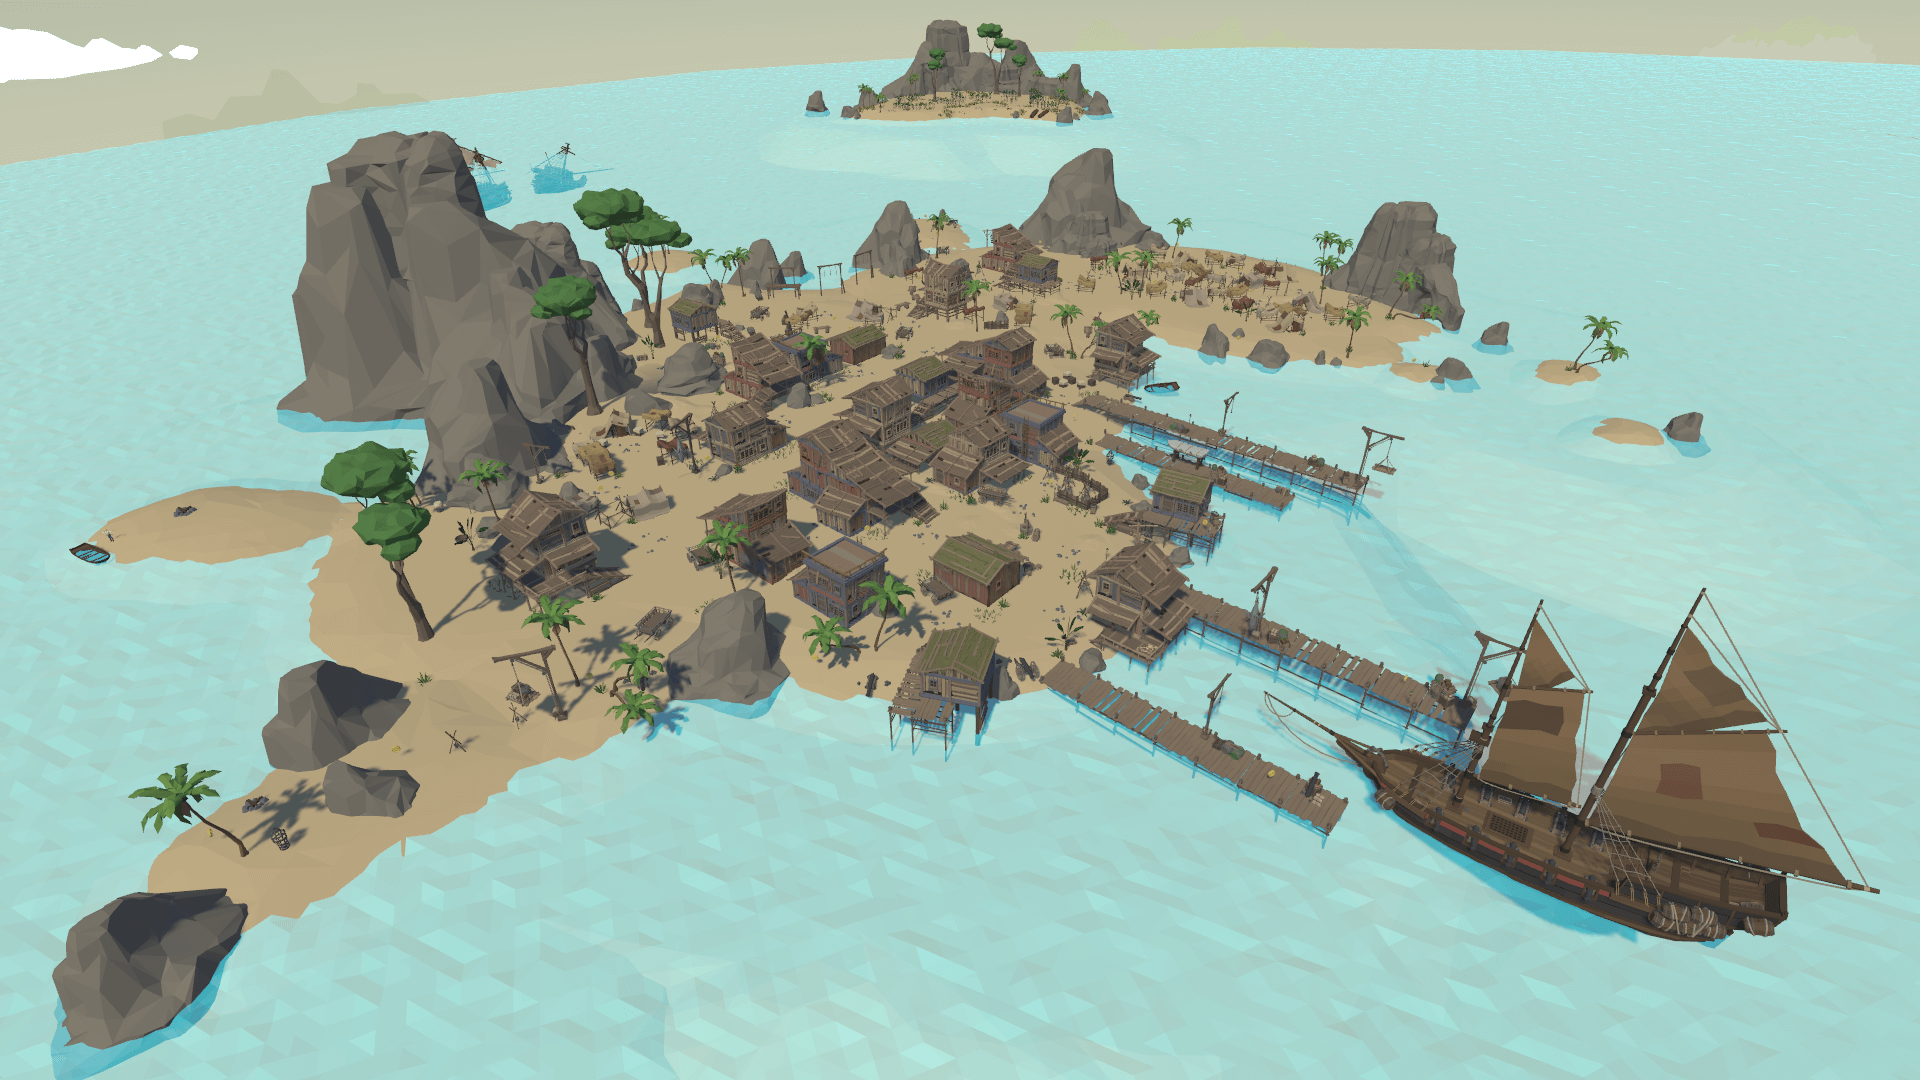
\includegraphics[width=.9\textwidth]{Figures/game_compressed.png}
    \caption{Herné prostredie}
    \label{pic:GameScreenshot}
\end{figure}

\section{Architektúra hry}
\label{sec:GameStructure}
Hra je rozdelená do dvoch samostatných scén. Konkrétne ide o hlavnú scénu, kde sa odohráva samotná herná slučka a scénu s hlavnou ponukou. V engine Unity je možné medzi jednotlivými scénami ľubovoľne prepínať, prípadne mať aktívnych niekoľko scén naraz. Každá scéna, ktorá je zahrnutá v builde má pridelené poradové číslo, tzv. build index, ktorý slúži aj ako jednoznačný identifikátor. Scéna s build indexom nula je potom spustená hneď po štarte aplikácie.

Scénu je potom možné chápať ako koreňový adresár pre hierarchiu objektov v hre. Jednotlivé herné objekty je možné vložiť do scény priamo, alebo ako potomka iného herného objektu. Manipulácia s pozíciou, rotáciou či mierkou objektu sa teda aplikuje aj na všetkých jeho potomkov. Naopak to však neplatí. Z tohto dôvodu sa rozlišujú dve súradnicové sústavy, a síce globálna (celková) a lokálna (relatívna voči predkovi). Využitie globálnej súradnicovej sústavy však vyžaduje vziať do úvahy parametre všetkých predkov daného objektu v scéne, čo nie je ideálne z hľadiska výkonu. Preto bol v projekte preferovaný lokálny súradnicový systém napríklad u herných NPC agentov či predmetov, ktoré je v hre možné zbierať. Predkovia týchto objektov sú potom umiestnení v počiatku súradnicovej sústavy, čo zaisťuje konzistenciu so zvyškom objektov v scéne.

V každej scéne sa nachádza objekt MainManager, ktorý slúži ako prístupový bod k ostatným manažérom, ktorí spravujú centrálne prvky hry. Tento typ architektúry sa kvôli svojej jednoduchosti často uplatňuje medzi malými až strednými projektami. V tomto projekte sú použité objekty ConfigManager, GameManager, InputManager a SoundManager, nie všetky sú však vyžadované v každej scéne. 

Krátky popis jednotlivých manažérov:
\begin{itemize}
  \item \textbf{ConfigManager} -- je prístupovým bodom k nastaveniam hry, zaisťuje serializáciu a deserializáciu dát, rovnako ako ich perzistentnosť po každej zmene.
  \item \textbf{GameManager} -- reštartuje scénu pri smrti alebo výhre hráča, kontroluje prerekvizity výhry, aktualizuje grafické užívateľské rozhranie pri získaní predmetu a zobrazuje kontextovú ponuku na ukončenie hry či návrat do hlavnej ponuky po stlačení príslušnej klávesy.
  \item \textbf{InputManager} -- centralizuje získavanie užívateľského vstupu z klávesnice, myši, či iných herných periférií, čo umožňuje na jednom centrálnom mieste zamieňať rôzne implementácie, prípadne z testovacích dôvodov hráčsky vstup úplne ignorovať. 
  \item \textbf{SoundManager} -- Vyvoláva jednoduchú simuláciu zvuku, na ktorú môžu zareagovať NPC agenti v dosahu.
\end{itemize}

\section{Herná slučka}
\label{sec:GameLoop}
Tradičná herná slučka definovaná napríklad podľa \cite{GameAlgorithms} sa skladá z troch fáz:

\begin{enumerate}
  \item Spracovanie vstupov
  \item Aktualizácia herného sveta
  \item Generovanie výstupov
\end{enumerate}

Hra teda prijme užívateľský vstup, na základe neho aktualizuje herný svet (dynamické objekty, ktoré sa v ňom vyskytujú) a výsledný stav je potom vyrenderovaný hráčovi v ďalšom snímku. Tento postup sa opakuje niekoľkokrát za sekundu, čo vyvoláva ilúziu dynamického sveta. Dnes sa považuje za štandard vykonanie hernej slučky 30 až 60 krát za sekundu. Dnešný hardvér však už podporuje vykresľovanie aj o rýchlosti 500FPS. Lepšou metrikou pre vývojárov je však tzv. frame time, teda trvanie jednej hernej slučky v ms. Vzťah týchto veličín je znázornený na obrázku \ref{pic:FrameTimeFPS}.

\begin{figure}[!htbp]
    \centering
    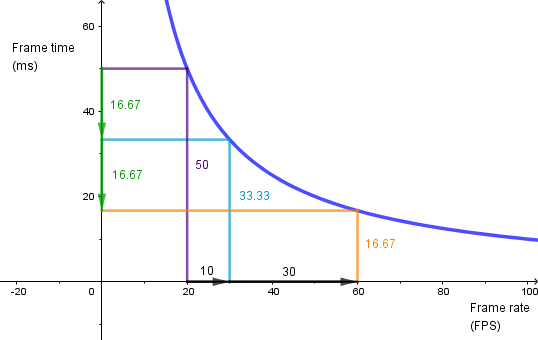
\includegraphics[width=.8\textwidth]{Figures/frameTimeVsFPS.png}
    \caption{Metriky Frame Time a FPS \cite{FrameTimeFPS}}
    \label{pic:FrameTimeFPS}
\end{figure}

V kontexte konkrétnej hry sa však pojem herná slučka alebo základná herná slučka (core game loop) využíva skôr na popis základných herných mechaník. V tomto prípade by teda šlo o prechod z bodu A do bodu B a zozbieranie určitého počtu predmetov na vymedzenej hernej ploche.

Pokiaľ hráčovi klesne život na nulu, hra pre neho končí a vracia sa na počiatočnú lokáciu. Nepriatelia a zberateľné predmety sa vrátia na svoje počiatočné pozície. Ak hráč dôjde do cieľa a splní prerekvizitu výhry, teda má v inventári určitý počet predmetov daného typu, hru vyhráva. Základnú hernú slučku obstaráva objekt GameManager spomenutý v sekcií \ref{sec:GameStructure}. 

Po hernej ploche je ručne rozmiestnených päť fliaš, z ktorých musí hráč nájsť a zobrať aspoň tri a tridsaťpäť mincí, pričom je pre dosiahnutie výhry nutné mať aspoň dvadsaťpäť. Implementačne oba typy objektov dedia z triedy Pickup, ktorej telo je možné vidieť vo výpise \ref{src:Pickup}. Tá potom dedí priamo z triedy UnityEngine.MonoBehaviour, čo je bázová trieda, z ktorej musia dediť všetky triedy, ktoré sú považované za Unity skripty. Unity skript môže potom využívať metódy životného cyklu ako napríklad Awake(), Start(), Update(), či FixedUpdate(), ale aj metódy sprístupňujúce prácu s korutinami apod. \cite{MonoBehaviour}.
\vspace{8pt}
\begin{lstlisting}[label=src:Pickup,caption={Trieda Pickup slúžiaca ako predok všetkých zberateľných predmetov v hre}]
public class Pickup : MonoBehaviour
{
    public event Action<Pickup> OnPickedUp;
    private WaitForEndOfFrame waitForFrameToEnd = new WaitForEndOfFrame();
    private MeshRenderer mesh;

    private void Start() 
    {
        MainManager.Instance.GameManager.RegisterPickup(this);
        mesh = GetComponentInChildren<MeshRenderer>();
    }
    
    private void OnTriggerEnter(Collider other) 
    {
        if (!other.gameObject.CompareTag(Constants.PlayerTag)) return;

        OnPickedUp?.Invoke(this);
        StartCoroutine(LerpPosition(transform.position, Camera.Instance.PickupTarget.position, 0.2f, () => { gameObject.SetActive(false); }));
    }
    
    private void OnDestroy() 
    {
        MainManager.Instance.GameManager.UnregisterPickup(this);
    }
    
    IEnumerator LerpPosition(Vector3 start, Vector3 end, float timeToMove, Action callback) 
    {
        float time = 0;

        while (time < 1)
        {
            mesh.transform.position = Vector3.Lerp(start, end, time);
            time += Time.deltaTime / timeToMove;

            yield return waitForFrameToEnd;
        }

        mesh.transform.position = end;
        callback();
    }
}
\end{lstlisting}

V metóde Start(), teda na začiatku svojho životného cyklu, ktorý sa odohrá po spustení scény sa každý zberateľný objekt zaregistruje v objekte GameManager, čo spôsobí napojenie na event OnPickedUp, a umožní GameManagerovi v správnej chvíli zareagovať na získanie predmetu hráčom a aktualizovať GUI či inventár bez nutnosti periodického dopytovania. Nakoľko je odberateľovi eventu odosielaná aj daná inštancia objektu, je jednoduché zistiť typ predmetu, ktorý hráč zobral.

Metóda OnTriggerEnter() je potom zavolaná v momente, keď hráčov kontroler začne kolidovať s komponentou Box Collider daného objektu. K tomu je nutné nastaviť tento Box Collider ako tzv. trigger a zároveň mať na objekte prítomnú komponentu Rigidbody, ktorá obstaráva simuláciu fyziky. V tomto momente sa zároveň pomocou korutiny LerpPosition() začne objekt rýchlo pohybovať do pravého horného rohu obrazovky, kde sa nachádza UI element zobrazujúci hráčovi počet zozbieraných predmetov, a následne sa deaktivuje. Tento efekt bol často využívaný v starších 2D platformových hrách. Zberateľný predmet je možné vidieť na obrázku \ref{pic:Pickup}.

\begin{figure}[!htbp]
    \centering
    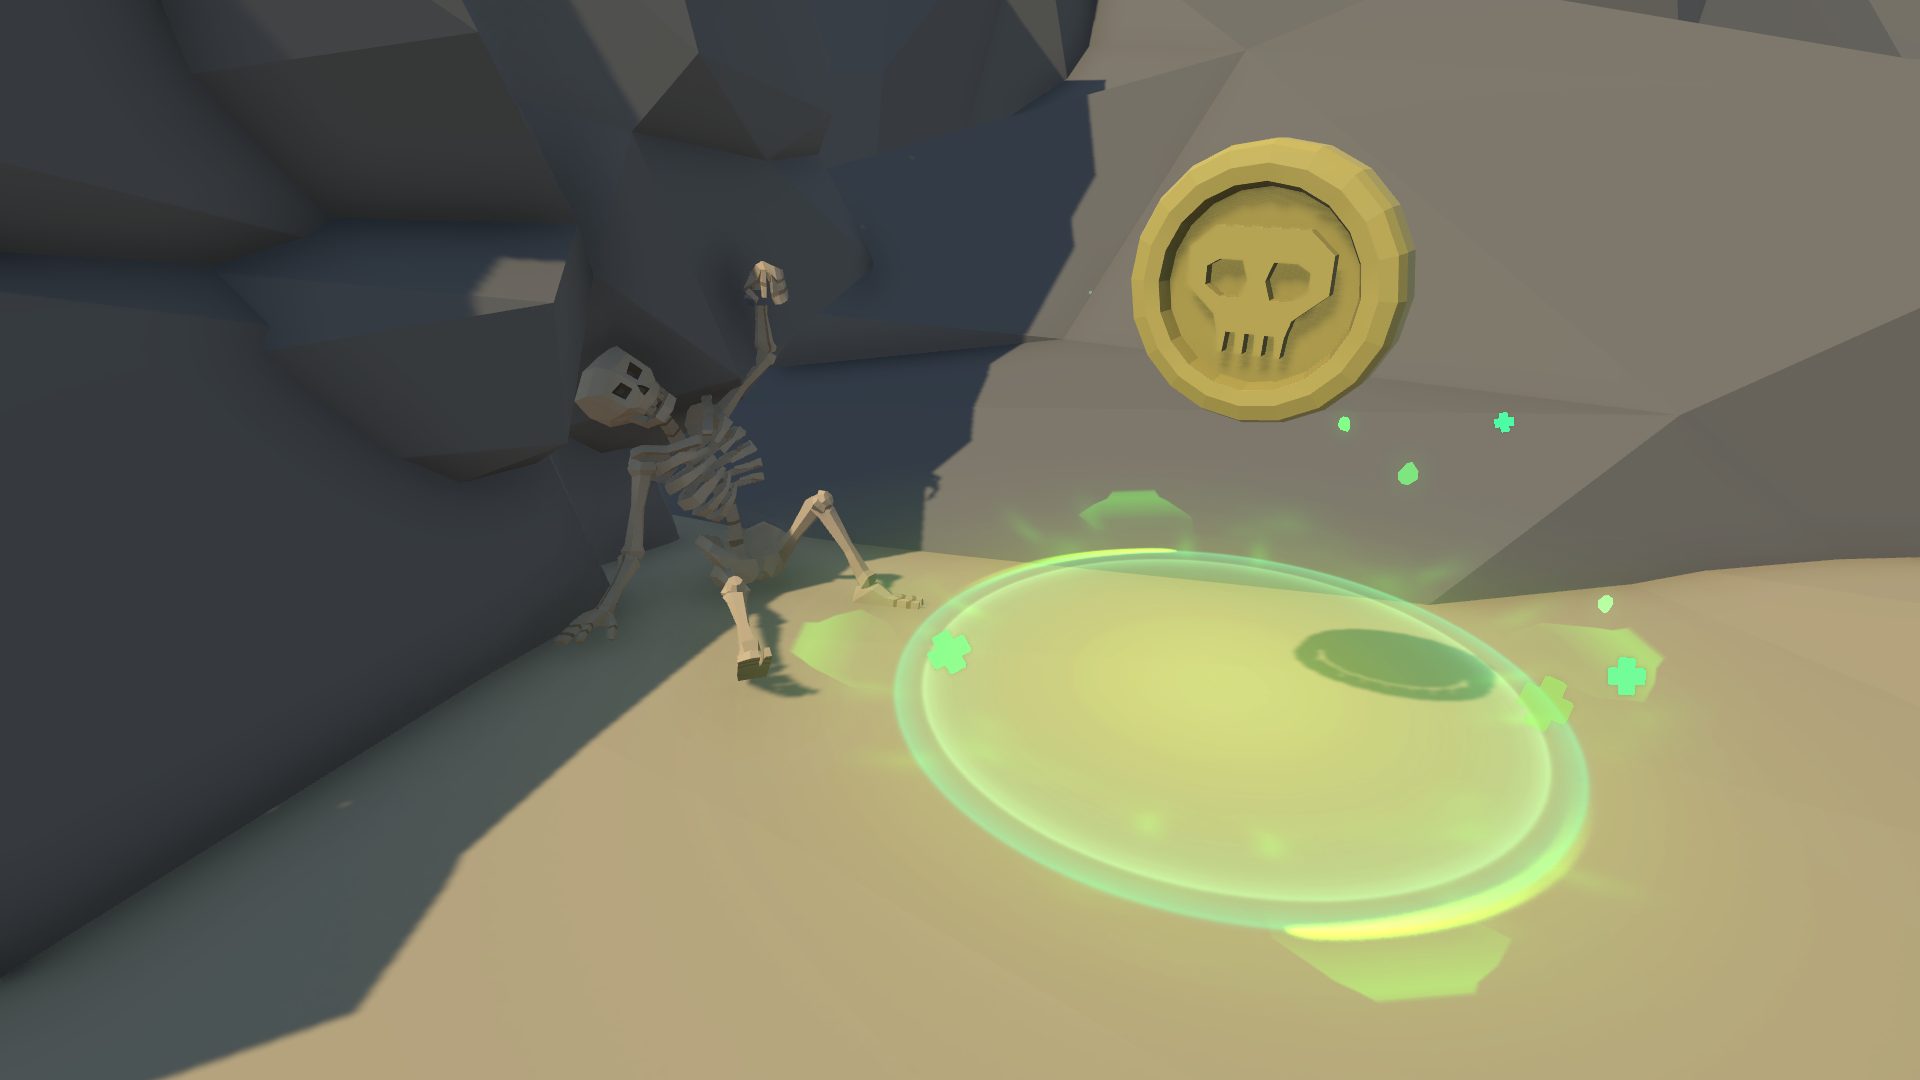
\includegraphics[width=.9\textwidth]{Figures/pickup.png}
    \caption{Zberateľný predmet minca}
    \label{pic:Pickup}
\end{figure}

Podobným spôsobom ako pri zberateľných predmetoch bola v projekte riešená aj interakcia s objektom Finish, ktorého úlohou je ukončiť hru v prípade, že s ním hráčov kontroler začne kolidovať. Taktiež teda obsahuje komponentu Box Collider nastavenú ako trigger a komponentu Rigidbody. Pri štarte hry sa tento Finish rovnako ako zberateľné predmety zaregistruje pod objekt GameManager a v metóde \mbox{OnTriggerEnter()}, po overení, že naozaj koliduje s hráčom, vyvolá event \mbox{OnTriggered}. Nakoľko bol Finish využívaný aj v trénovacej fáze, bol pre tento účel vytvorený jednoduchý interface IFinish obsahujúci spomínanú metódu OnTriggered a jeho dve implementácie: FinishGame a FinshEpisode. Prvá implementácia je využívaná v hlavnej scéne a ukončuje hru, druhá, ako názov napovedá, ukončuje trénovaciu epizódu v neprospech AI agenta. Táto problematika je bližšie popísaná v kapitole \ref{sec:Training}.

Po vyvolaní spomínaného eventu objekt GameManager overí prerekvizity výhry a pokiaľ ich hráč spĺňa ukončí hru. Tento postup je možné vidieť vo výpise \ref{src:FinishGame}. Pomocou eventu OnGameFinished zároveň všetkým odberateľom oznámi ukončenie hry. Najdôležitejší odberatelia eventu sú herná kamera a pohybový systém hráča, ktorí okamžite zastavia svoju činnosť a stanú sa pasívnymi. Zároveň s týmto sa hráčovi začne postupne zobrazovať informácia o úspešnom dokončení hry a po určitej dobe sa reštartuje scéna, čo umožní hráčovi skúsiť to znova napríklad s inými parametrami.

\vspace{8pt}
\begin{lstlisting}[label=src:FinishGame,caption={Ukončenie hry v prípade výhry hráča}]
private bool PrerequisitesMet()
{
    return (pickedBottles >= minBottles) && (pickedCoins >= minCoins);
}
private void GameFinished()
{
    if (!PrerequisitesMet())
    {
        ShowPrerequisitesNotMetInfo();
        return;
    }

    OnGameFinished?.Invoke();

    if (youWonUI != null)
        youWonUI.SetActive(true);

    StartCoroutine(RestartSceneCoroutine());
}
private IEnumerator RestartSceneCoroutine()
{
    yield return uiWait;
    SceneManager.LoadScene(SceneManager.GetActiveScene().name);
}
\end{lstlisting}

Medzi ďalšie kompetencie GameManagera patrí na základe nastavení uložených v objekte ConfigManager inštancovať pri štarte hry NPC agentov určeného typu na konkrétne pozície a rotácie. Bližší popis štruktúry agentov, ich inštancovanie a fungovanie je popísané v sekcií \ref{sec:Agents}.

Poslednou kompetenciou GameManagera je periodicky v rámci metódy OnUpdate() zisťovať od objektu InputManager, či bola stlačená klávesa na pozastavenie hry a na základe toho zobraziť hráčovi príslušný GUI element. Tento postup bol zvolený z dôvodu, že vstavaný input systém enginu Unity nedokáže spracovávať užívateľský vstup tzv. event-driven prístupom. Spomínaný GUI element je možné vidieť na obrázku \ref{pic:PauseUI} a umožňuje hráčovi rozhodnúť, či chce ukončiť hru alebo sa vrátiť do hlavnej ponuky. 

\begin{figure}[!htbp]
    \centering
    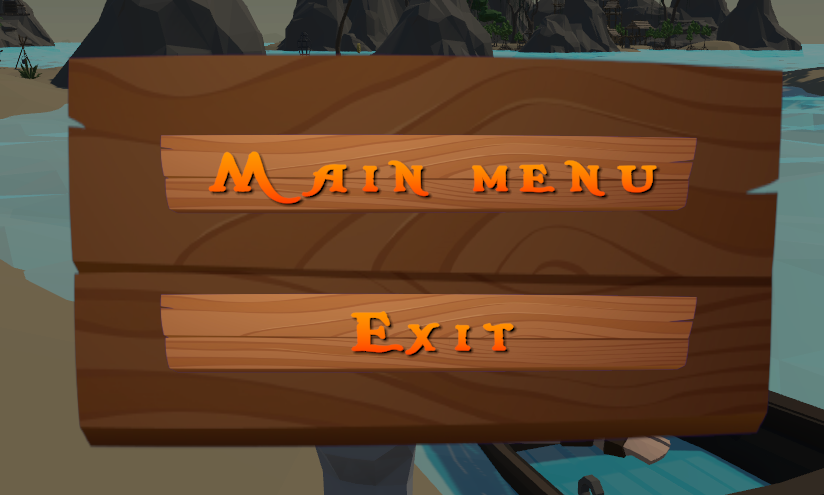
\includegraphics[width=.65\textwidth]{Figures/pauseUI.png}
    \caption{GUI element s umožňujúci návrat do hlavnej ponuky alebo ukončenia hry}
    \label{pic:PauseUI}
\end{figure}

Obe tlačidlá na GUI elemente zobrazenom na obrázku \ref{pic:PauseUI} obsahujú Unity komponentu Button, ktorá vie napríklad zmeniť farebnú schému elementu, keď nad ním hráč nadíde myšou. Dôležitejšou funkcionalitou je však možnosť priradiť eventu OnClick ľubovoľný objekt priamo v editore a interakcia s tlačidlom dokáže zavolať na tomto objekte určenú verejnú metódu, čo demonštruje obrázok \ref{pic:OnClick}. 

\begin{figure}[!htbp]
    \centering
    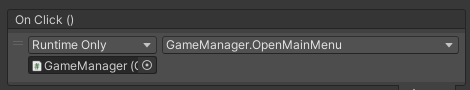
\includegraphics[width=.8\textwidth]{Figures/OnClick.png}
    \caption{Nastavenie OnClick eventu tlačidla v editore}
    \label{pic:OnClick}
\end{figure}

V tomto prípade bol tlačidlám predaný objekt GameManager a volané boli jeho dve verejné metódy OpenMainMenu() a QuitGame() zobrazené vo výpise \ref{src:MMQuit}.

\vspace{8pt}
\begin{lstlisting}[label=src:MMQuit,caption={Metódy na návrat do hlavnej ponuky a ukončenie hry}]
public void OpenMainMenu()
{
    SceneManager.LoadScene(0);
}
public void QuitGame()
{
#if UNITY_EDITOR
    UnityEditor.EditorApplication.isPlaying = false;
#endif
    Application.Quit();
}
\end{lstlisting}

Metóda OpenMainMenu() načíta scénu s build indexom nula. Tento postup je vhodné aplikovať pri fixne danom poradí scén v zostavení aplikácie. Zamedzí sa tým zbytočnému prehľadávaniu scén podľa mena. Poradie scén v rámci tohto projektu je popísané v sekcií \ref{sec:GameStructure}. 

Ukončenie hry potom prebieha jednoduchým zavolaním metódy Application.Quit(). Tento prístup však nefunguje na aplikáciu spustenú v editore Unity. Z tohto dôvodu je v rámci direktivy preprocesoru UNITY\_EDITOR, nutné aj nastavenie premennej isPlaying v triede UnityEditor.EditorApplication na hodnotu false. 

Direktívy preprocesoru v jazyku C\# umožňujú selektívne zahrnúť alebo vylúčiť kód z kompilácie na základe toho, či sú alebo nie sú definované určité skriptovacie symboly. Engine Unity ná na tieto účely preddefinované symboly umožňujúce rozlíšiť rôzne platformy či práve zostavenie aplikácie od behu v editore \cite{ConditionalCompilation}.

\section{Hlavná ponuka hry}
\label{sec:MainMenuAndUI}

Ako už bolo spomenuté v predchádzajúcich sekciách vytvorená hra obsahuje scénu s hlavnou ponukou. Táto scéna obsahuje informačnú tabuľu s aktuálnymi nastaveniami a štyri aktívne prvky užívateľského rozhrania. Ide o tlačidlá Play, Options, Credits a Exit. Tieto tlačidlá opäť obsahujú Unity komponentu Button a referenciu na objekt, ktorého verejné metódy volajú. Hlavnú ponuku je možné vidieť na obrázku \ref{pic:MainMenu}.

\begin{figure}[!htbp]
    \centering
    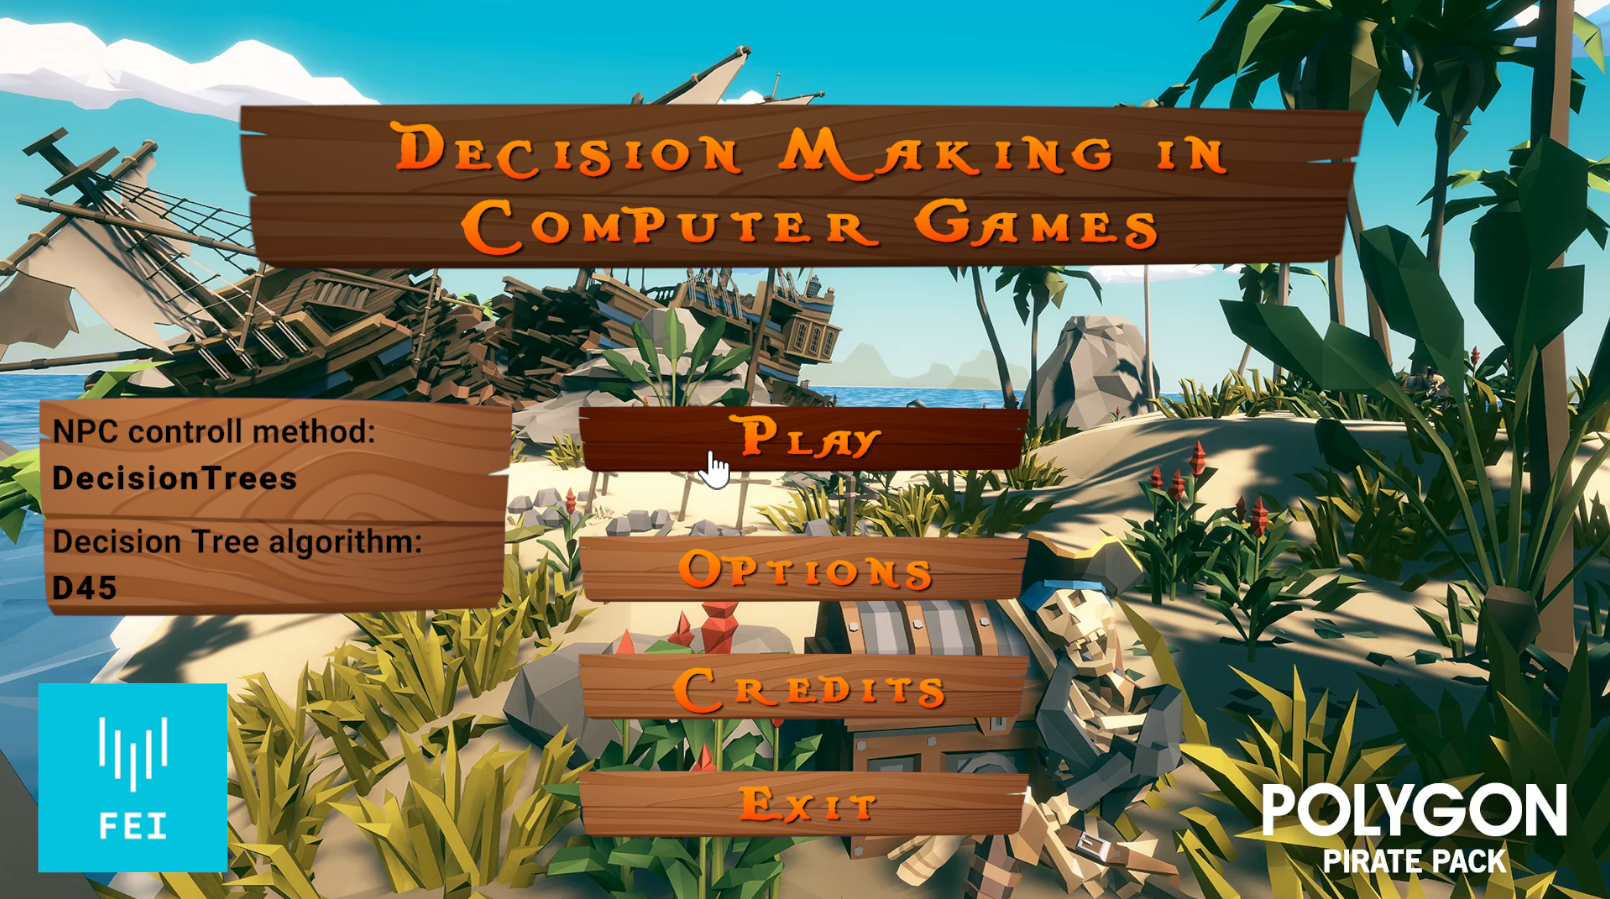
\includegraphics[width=.9\textwidth]{Figures/mainMenu.png}
    \caption{Hlavná ponuka hry}
    \label{pic:MainMenu}
\end{figure}

Informačná tabuľa na ľavej strane obrazovky zobrazuje, či budú NPC agenti v hre ovládaní rozhodovacím stromom alebo pomocou Reinforcement learningu. Pokiaľ budú agenti ovládaní pomocou rozhodovacieho stromu, v spodnej časti tabule sa zobrazí aj algoritmus, ktorým má byť strom zostrojený. Tieto nastavenia sú perzistentné a teda ostanú uchované aj po vypnutí aplikácie. Zmeny je možné vykonať v ponuke Options. Stlačenie príslušného tlačidla v tejto ponuke vyvolá zmenu na objekte ConfigManager. Ten pomocou jednoduchej metódy Serialize() tieto zmeny aktualizuje na disku v súbore \textit{settings.txt} uloženom v adresári danom premennou \textit{Application.persistentDataPath}. Konkrétna cesta sa líši v závislosti od aktuálnej platformy. Zároveň je zmena v dátach propagovaná pomocou eventu OnDataChanged, ktorého odberateľom je hlavná ponuka, ktorá tieto zmeny aktualizuje v informačnej tabuli.

Tlačidlo Exit ukončí beh aplikácie a tlačidlo Play spustí hlavnú scénu hry. Obdobná funkcionalita bola demonštrovaná už vo výpise \ref{src:MMQuit}.

Tlačidlo Credits zavolá metódu SetActive() so vstupným parametrom nastaveným na false na svojom predkovi, ktorý združuje všetky tlačidlá, informačnú tabuľu a tabuľu s menom aktuálnej ponuky. Zároveň obdobným spôsobom aktivuje ponuku Credits, ktorá mu bola referencovaná v editore. 

Tlačidlo Options potom využíva rovnaký prístup na zobrazenie ponuky s výberom typu NPC agenta proti ktorému chce hráč hrať. V prípade, že hráč vyberie možnosť Decision Trees je mu ešte zobrazená ponuka s výberom algoritmu, ktorý chce použiť na zostavenie rozhodovacieho stromu.

Každá vnorená ponuka, ktorá sa stane aktívna sa začne periodicky dopytovať objektu InputManager, či bola stlačená príslušná klávesa na návrat do predchádzajúcej ponuky. Na tento účel bola vytvorená jednoduchá trieda zobrazená vo výpise \ref{src:SubMenu}.

\vspace{8pt}
\begin{lstlisting}[label=src:SubMenu,caption={Trieda SubMenu}]
public class SubMenu : MonoBehaviour
{
    [SerializeField]
    private GameObject currentSubMenu;
    [SerializeField]
    private GameObject previousSubMenu;

    private void Update()
    {
        if (MainManager.Instance.InputManager.WasCancelledLastFrame)
        {
            currentSubMenu.SetActive(false);
            previousSubMenu.SetActive(true);
        }
    }
}
\end{lstlisting}

Jednotlivé ponuky sú v triede referencované pomocou atribútu \textit{SerializeField} a na jednotlivých objektoch boli nastavené ručne v editore. Atribút \textit{SerializeField} vynúti serializáciu u neverejných členských premenných \cite{SerializeField}, čím sa neporušuje princíp zapuzdrenia a zároveň to umožňuje jednoducho referencovať medzi sebou objekty priamo v editore Unity pomocou tzv. Drag \& Drop či výberu z rolovacej ponuky. Nie je teda nutné prehľadávať objekty v scéne alebo riešiť prístup k danému objektu architektonicky na úrovni kódu. Tento prístup však nie je možné použiť na prepojenie dvoch objektov, pričom jeden z nich je prítomný v scéne od začiatku a druhý je inštancovaný za behu aplikácie. Všetky jednotlivé ponuky sú súčasťou hierarchie scény od jej spustenia, takže nebol s týmto prístupom problém. Diagram všetkých ponúk je možné vidieť na obrázku \ref{pic:MainMenuScheme}.

\begin{figure}[!htbp]
	\centering
	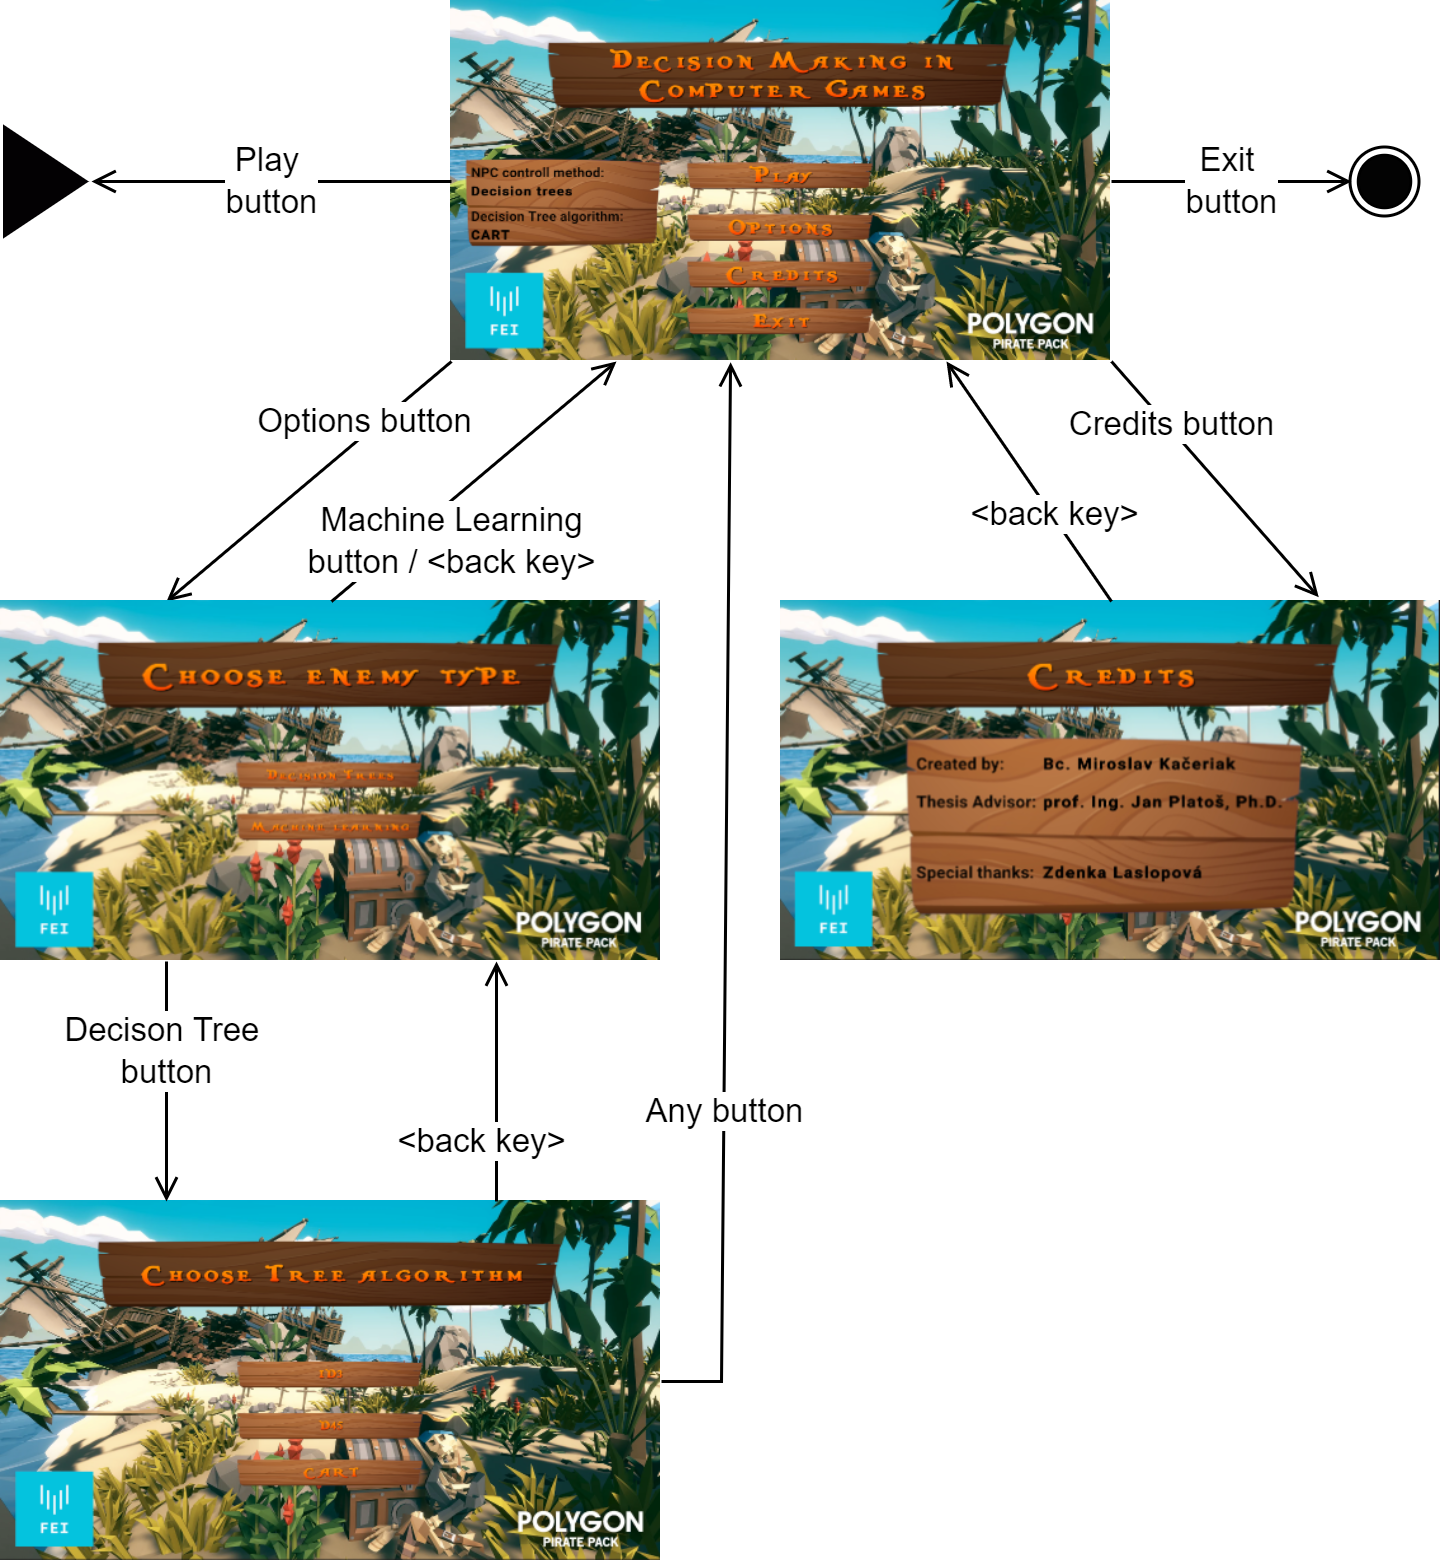
\includegraphics[width=.85\textwidth]{Figures/mainMenuScheme.png}
	\caption{Diagram obrazoviek hlavnej ponuky}
	\label{pic:MainMenuScheme}
\end{figure}

% Chapter 5
\chapter{Architektúra hráčskej postavy}
\label{sec:Player}
Jednou z najdôležitejších súčasti hier ovládaných z pohľadu tretej osoby je práve hráčska postava. Tá reaguje na hráčov vstup zmenou smeru alebo rýchlosti pohybu, akciami ako skok, útok, úhyb či kontextuálnou interakciou s nejakým objektom v hre a podobne. Na postavu hráča pôsobí určitá forma gravitácie a s tým súvisiaca kolízia s hernou plochou a ostatnými statickými či dynamickými objektami. Hráčska postava má spravidla nastavenú nejakú hodnotu zdravia či života, ktorá sa v čase mení napríklad po páde z veľkej výšky či po zásahu od nepriateľa. Hodnota ostávajúceho zdravia je často hráčovi prezentovaná vo forme GUI ukazovateľa. 

Táto kapitola popisuje akým spôsobom bolo k jednotlivým problémom pristupované v tomto projekte. Niektoré princípy je možné s väčšími či menšími úpravami aplikovať obecne, iné sú poplatné enginu Unity. 

\section{Prehľad komponentov}
\label{sec:PlayerComponentOverview} 
Samotný objekt hráčskej postavy sa skladá z dvoch objektov, ktoré sa zvyknú nazývať kontroler a model. 

Model reprezentuje vizuálnu stránku objektu, teda postavu samotnú a ďalšie menšie objekty, ktoré má táto postava na sebe. Pri zložitejších modeloch ide o hierarchiu čítajúcu stovky objektov reprezentujúce jednotlivé časti tela. V tomto prípade je využitý tzv. low poly model, ktorý je vcelku a pod sebou má iba zopár vizuálnych doplnkov, ktoré postava nosí okolo pása. Low poly modely hráčskej postavy, nepriateľov a prostredia pochádzajú z balíka POLYGON Pirates od spoločnosti Synty Studios zakúpeného v oficiálnom online obchode enginu Unity \cite{Synty}.

Kontroler, na druhú stranu obsahuje sadu komponentov, ktoré obstarávajú pohyb, gravitáciu, kolíziu a ľubovoľnú ďalšiu funkcionalitu. Dôležitou súčasťou kontrolera je práve Unity komponenta Character Controller. Na nej je možné nastaviť rôzne parametre definujúce tvar kolíznej kapsule, maximálnu výšku kroku, ktorý môže postava vykonať bez nutnosti vyskočiť apod. Túto kapsulu s kompletnou vizuálnou stránkou hráča je možné vidieť na obrázku \ref{pic:PlayerController}.

\begin{figure}[!htbp]
	\centering
	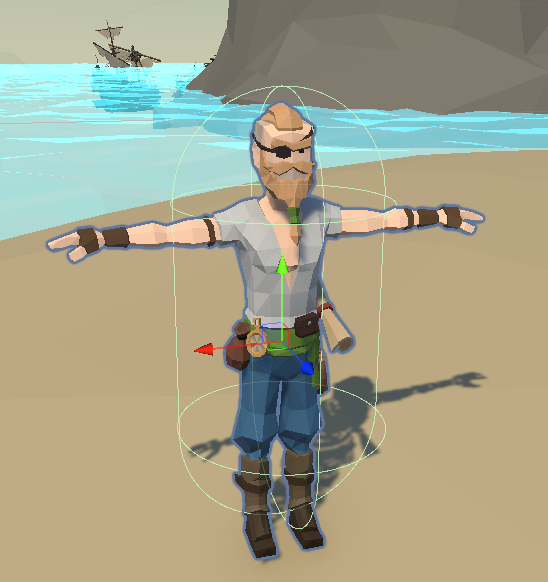
\includegraphics[width=0.54\textwidth]{Figures/controller.png}
	\caption{Hráčka postava s komponentou Character Controller}
	\label{pic:PlayerController}
\end{figure}

Na objekte kontroler sa ďalej nachádzajú komponenty PlayerBrain, PlayerBody, PlayerMovement, PlayerAutomaticMovement a NavMeshAgent. Posledné dve spomenuté komponenty sú v predvolenom stave deaktivované a aktivuje ich komponenta PlayerBrain v prípade, že má objekt ConfigManager v editore nastavenú premennú PlayerControll na hodnotu Automatic. Toto je využívané primárne v trénovacích scenároch, ktoré sú bližšie popísané v sekcií \ref{sec:Training}. V tomto prípade taktiež komponenta PlayerBrain vypne komponentu PlayerMovement, čím znemožní ovládať hráča pomocou vstupu z periférií. 

Poslednou kompetenciou komponenty PlayerBrain je držať referencie na zvyšné komponenty a inicializovať ich. Počas inicializačnej fázy sú jednotlivým komponentám predané referencie na iné komponenty ktoré potrebujú pre svoje fungovanie. Tento prístup umožňuje centrálne riadiť prepojenia medzi komponentami bez nutnosti ich rôzne referencovať navzájom v editore.

\section{Prijímanie poškodenia}
\label{sec:DealingDamage}
Hráčska postava je zraniteľná voči útoku nepriateľského NPC agenta. Maximálna hodnota poškodenia, ktorú hráčska postava môže inkasovať kým zomrie je nastavená v komponente PlayerBody. Táto komponenta teda obsahuje maximálnu hodnotu zdravia, ktorá sa hráčovi nastaví na začiatku hry a aktuálnu hodnotu zdravia, ktorá klesá s prijímaným poškodením. Všetká potrebná funkcionalita súvisiaca s prijímaním poškodenia vrátane propagovania informácie o zmene hodnoty zdravia či smrti danej postavy bola zjednotená pod rozhranie IDamageable. Toto rozhranie okrem komponenty PlayerBody implementuje aj abstraktná komponenta NPCBody, ktorá bude bližšie popísaná v sekcií \ref{sec:Agents}. Spomínané rozhranie je možné vidieť vo výpise \ref{src:IDamageable}. 

\vspace{8pt}
\begin{lstlisting}[label=src:IDamageable,caption={Rohranie IDamageable}]
public interface IDamageable
{
    public float MaxHealth { get; }
    public float Health { get; }

    public event Action<float> OnHealthChanged;
    public event Action OnDied;

    public void DealDamage(float damage);
}
\end{lstlisting}

Komponenta PlayerBody sa pri spustení hry zaregistruje pod objekt GameManager ako implementácia rozhrania IDamageable. GameManager sa v tomto momente stane odberateľom eventu OnHealthChanged za účelom aktualizácie GUI elementu zobrazujúceho aktuálny stav zdravia hráčskej postavy. Tento element sa zvykne nazývať Health bar.

Zavolanie metódy DealDamage() na hráčskej postave teda spôsobí odrátanie hodnoty poškodenia od aktuálnej hodnoty zdravia a vyvolanie spomínaného eventu. Pokiaľ táto hodnota zdravia klesne na nulu je na hráčskej postave deaktivované ovládanie pohybu a vyvolá sa event OnDied. Na tento event zareaguje odberateľ GameManager, ktorý vyvolá event OnGameEnded, na základe ktorého sa deaktivuje ovládanie kamery a následne je hráčovi zobrazená informácia o konci hry. Po určitom čase je scéna reštartovaná a hráč to môže skúsiť znova a lepšie. 

Informáciu o konci hry spolu s prázdnym GUI elementom Health bar je možné vidieť na obrázku \ref{pic:YouDied}. Na tomto obrázku je možné povšimnúť si aj GUI elementy zobrazujúce hráčovi počet nazbieraných predmetov spolu s minimálnym počtom, ktorý je vyžadovaný na úspešné dokončenie hry. Aktualizácia počtu zozbieraných predmetov v GUI záležitosťou nastavenia reťazca v premennej text príslušného objektu. 

\begin{figure}[!htbp]
	\centering
	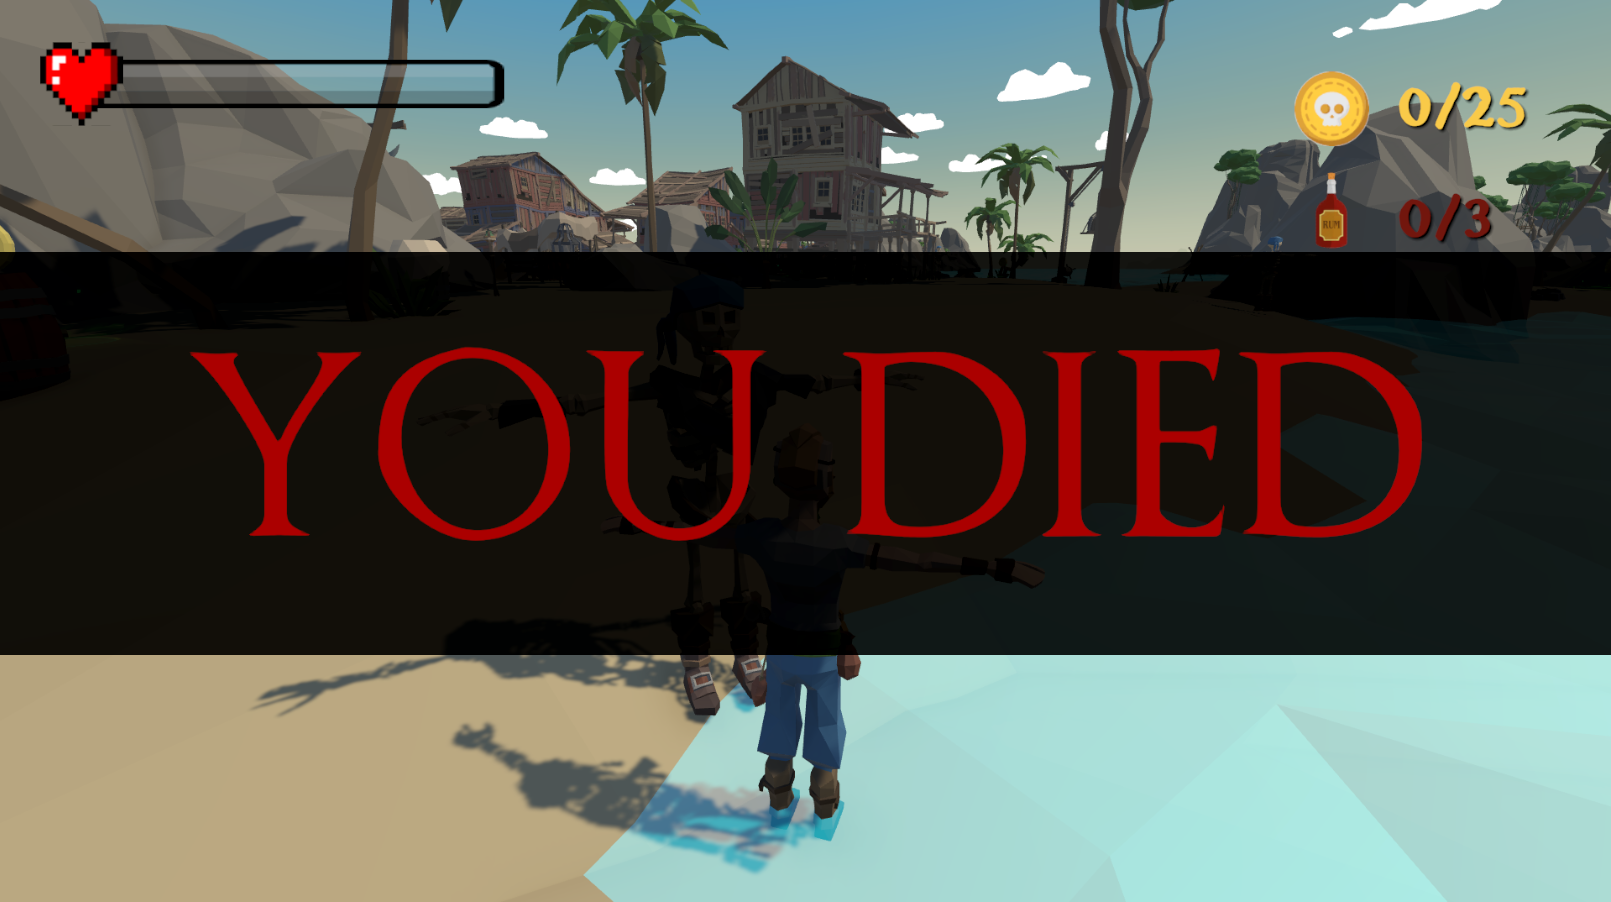
\includegraphics[width=.8\textwidth]{Figures/youDied.png}
	\caption{GUI elementy v hlavnej scéne}
	\label{pic:YouDied}
\end{figure}

GUI element Health bar sa skladá z troch častí: výplň, obrys a ikona srdca. Na aktualizáciu hodnoty v tomto GUI elemente je využívaná Unity komponenta Slider. Táto komponenta má množstvo nastavení a parametrov vrátane objektu, ktorého rozmery bude Slider ovplyvňovať (v tomto prípade výplň elementu) a maximálnej hodnoty. Tá sa pri spustení hry nastaví na hodnotu maximálneho zdravia hráčskej postavy a je teda možné priamo bez prepočtu nastavovať hodnotu Slideru v reakcii na zmenu zdravia hráča.

\section{Pohyb}
\label{sec:PlayerMovement} 
Jednou z najdôležitejších súčastí hráčskej postavy je práve možnosť jej ovládania pomocou periférií. Pre tento účel bola vytvorená komponenta PlayerMovement. Táto komponenta teda periodicky obstaráva komunikáciu s objektom InputManager, z ktorého získané vstupy transformuje na pohyb postavy v trojrozmernom hernom priestore pomocou komponenty Character Controller.

Existuje množstvo prístupov k tejto problematike a v závislosti od typu hry či členitosti herného prostredia môže byť práve pohyb hráča veľmi komplexnou témou hlavne v kombinácií s realistickými animáciami.

V tomto projekte bol využitý základný systém využívajúci možností vstavanej Unity komponenty Character Controller a to ako na pohyb tak aj na zisťovanie, či sa hráč nachádza na pevnej zemi. Hráčovi je okrem základného pohybu do rôznych smerov umožnené skákať, či spomaliť svoj pohyb, čím sa zníži rozsah šírenia zvuku jeho krokov. Pohyb hráča taktiež podlieha základnej simulácií gravitácie. Metódu Update() komponenty PlayerMovement, ktorá obstaráva vyššie popísanú funkcionalitu je možné vidieť vo výpise \ref{src:PlayerMovement}.

\vspace{8pt}
\begin{lstlisting}[label=src:PlayerMovement,caption={Metódy komponenty PlayerMovement obstarávajúce pohyb hráčskej postavy}]
void Update()
{
    var currentSpeed = speed;

    if (controller.isGrounded)
        UpdateGrounded(ref currentSpeed);

    Vector3 direction = new Vector3(horizontal, 0, vertical);
    float magnitude = Mathf.Clamp01(direction.magnitude) * currentSpeed;
    direction.Normalize();

    float angle = SmoothAngleFromDirection(direction);
    if (direction != Vector3.zero)
        transform.localRotation = Quaternion.Euler(0f, angle, 0f);

    Vector3 moveDirection = Quaternion.Euler(0f, angle, 0f) * Vector3.forward;
    Vector3 velocity = moveDirection.normalized * magnitude;

    ySpeed += Physics.gravity.y * Time.deltaTime;
    velocity.y = ySpeed;

    controller.Move(velocity * Time.deltaTime);
    MakeNoise(velocity);
}
private void UpdateGrounded(ref float currentSpeed)
{
    ySpeed = defaultYSpeed;

    horizontal = inputManager.Horizontal;
    vertical = inputManager.Vertical;

    if (inputManager.WasJumpingThisFrame)
        ySpeed = jumpSpeed;

    if (inputManager.IsCrounching)
        currentSpeed /= 2;
}
\end{lstlisting}

Vo výpise \ref{src:PlayerMovement} je možné si povšimnúť, že pokiaľ sa hráčska postava nachádza na zemi, je možné zmeniť jej smer na osách X a Z, vyskočiť, či znížiť rýchlosť pohybu na polovicu, čo sa prejaví pri šírení zvuku krokov. V tomto prípade je aj vyresetovaná rýchlosť postavy na ose Y a to na nulu. V momente kedy hráč stlačí tlačidlo skoku, je táto rýchlosť nastavená na hodnotu výšky skoku a počas nasledujúcich snímkov bude klesať rýchlosťou danou hodnotou gravitačnej konštanty vynásobenej časom medzi jednotlivými snímkami. Keď postava dopadne na zem je táto rýchlosť opäť vyresetovaná a medzi jednotlivými snímkami sa mení len minimálne v závislosti na hodnote FPS a teda mierne tlačí postavu k zemi, čím sa eliminujú problémy s prípadnou zlou detekciu zeme pri nerovnom teréne.

Následne sa na základe hráčskeho vstupu vypočíta smer a rýchlosť pohybu, ktorým sa má postava vydať a výsledná hodnota, opäť vynásobená časom medzi jednotlivými snímkami, je odoslaná do metódy Move() komponenty Character Controller. Táto metóda vykoná pohyb postavy, pokiaľ to kolízna kapsula či výška nerovného terénu dovolí. Násobenie hodnotou Time.deltaTime, teda časom medzi jednotlivými snímkami spôsobí, že rýchlosť pohybu bude nezávislá od snímkovej frekvencie hry.

Taktiež je vhodné neaplikovať smer na rotáciu postavy priamo, ale vziať do úvahy aktuálnu rotáciu kamery, teda smer, do ktorého sa hráč pozerá. Z dôvodu eliminácie instantnej zmeny rotácie, čo spôsobí nepríjemný efekt teleportácie modelu do daného smeru je tiež vhodné robiť veľké zmeny postupne. Tento prístup je znázornený vo výpise \ref{src:SmoothAngleFromDirection}.

\vspace{8pt}
\begin{lstlisting}[label=src:SmoothAngleFromDirection,caption={Postupná zmena rotácie postavy v súlade s rotáciu kamery}]
private float SmoothAngleFromDirection(Vector3 direction)
{
    var cameraY = (cameraTransform == null) ? 
    cameraTransform.eulerAngles.y : 0.0f;

    float tempAngle = Mathf.Atan2(direction.x, direction.z) * Mathf.Rad2Deg + cameraY;
    return Mathf.SmoothDampAngle(transform.eulerAngles.y, tempAngle, ref turnSmoothVelocity, turnSmoothTime);
}
\end{lstlisting}

Poslednou kompetenciou komponenty PlayerMovement je vydávanie zvuku pri pohybe. To je realizované pomocou metódy MakeNoise() vo výpise \ref{src:PlayerMovement}. Táto metóda na základe vstupného parametru, ktorý reprezentuje rýchlosť pohybu vypočíta druhú mocninu dĺžky X a Z zložky vstupného vektoru. Tú spolu s aktuálnou pozíciou vloží ako parametre koštruktora readOnly štruktúry Noise a následne zavolá na objekte SoundManager metódu MakeNoise, ktorej danú inštanciu štruktúry odošle ako parameter. Tento postup sa vykonáva v pravidelných intervaloch, ktorých dĺžka je daná konštantou stepDelay a za splnenia podmienky, že hráč nie je statický. 

SoundManager následne vytvorí tzv. SphereCast a teda získa všetky kolidery v rádiuse daného bodu v priestore. Všetky nájdené objekty sú skontrolované na prítomnosť komponenty Hearing. Ak objekt obsahuje túto komponentu je na nej zavolaná metóda RespondToNoise(), ktorej je predaná pozícia danej inštancie zvuku. Reakcia na tento podnet je bližšie popísaná v kapitole \ref{sec:Agents}. Pomocou Unity metódy OnDrawGizmosSelected() bola taktiež v editore vytvorená jednoduchá vizualizácia zvuku za účelom ladenia

\section{Kamera}
\label{sec:Camera}

Kamera je veľmi dôležitým prvkom každej hry. Nielenže hráč pomocou nej môže sledovať dianie v hernom svete ale už samotným pohybom tejto kamery môže ovplyvňovať napríklad smer pohybu hráčskej postavy, čo bolo demonštrované v predchádzajúcej sekcií. 

V editore Unity je možné využiť na snímanie diania v hre predpripravenú komponentu Camera. Tá umožňuje nastavenie rôznych parametrov od FOV, typu projekcie, vzdialenosti orezávacích rovín až po napríklad anti-aliasing. Bez prítomnosti kamery v scéne je renderovaná iba čierna obrazovka s varovným nápisom a GUI. Kamier v scéne môže byť niekoľko a je možné medzi nimi plynulo prepínať napríklad v rámci filmových sekvencií čí mierenia so zbraňou.

Ovládanie kamery bolo realizované pomocou modulu Cinemachine od spločonosťou Unity, ktorá vytvára aj samotný engine. Tento modul je zdarma dostupný z oficiálneho repozitára a obsahuje niekoľko typov kamier, ktoré je možné použiť. V tomto projekte je využitá tzv. Free Look Camera. Po výbere kamery je na objekt obsahujúci Unity komponentu Camera pridaná komponenta z tohto modulu s názvom CinemachineBrain a následne je vytvorený nový herný objekt, ktorý obsahuje komponentu s názvom odpovedajúcim vybranému typu kamery. Komponenta CinemachineBrain sa prepojí s komponentou tohto nového objektu, a ten prevezme kontrolu nad pozíciou a rotáciou pôvodnej kamery bez nutnosti ručného nastavovania týchto parametrov zo skriptu.

\begin{figure}[!htbp]
    \centering
    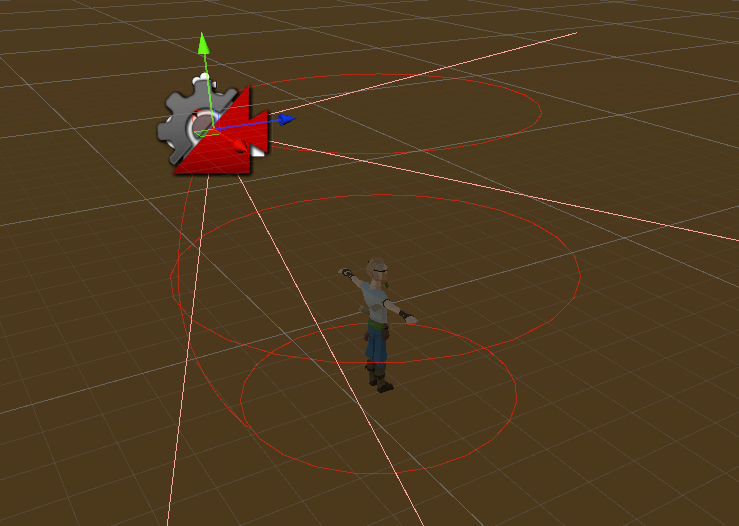
\includegraphics[width=.7\textwidth]{Figures/obruce.png}
    \caption{Vizualizácia obručí, po ktorých sa pohybuje herná kamera}
    \label{pic:Cinemachine}
\end{figure}

Komponenta ovládajúca kameru má veľké množstvo nastavení, ktorých popis by presahoval rámec tejto práce. Dôležitým parametrami sú hlavne referencie na objekt, ktorý má kamera prenasledovať a na ktorý sa má zamerať. V tomto prípade bola na oba prípady použitá referencia hráčskej postavy. Ďalej boli na tomto mieste nastavené rýchlosti či rozsah pohybu kamery na jednotlivých osách, ktoré boli zároveň namapované na príslušné osy vstupných periférií. Kvôli kolízií kamery s hernými objektami bola ešte pridaná a nastavená komponenta Cinemachine Collider.

Samotná kamera sa potom pohybuje po troch obručiach - spodnej, strednej a hornej. Výšku a priemer týchto obručí je taktiež možné upraviť a každá z nich má separátne nastavenia, ktoré určujú stred pohľadu kamery, mŕtvu zónu, rýchlosť s akou sa kamera snaží dohnať svoj cieľ apod. Tieto obruče sú pre lepšiu predstavu znázornené na obrázku \ref{pic:Cinemachine}.

%Chapter 6
\chapter{Architektúra NPC agentov}
\label{sec:Agents}
Ako už bolo spomenuté v predchádzajúcich kapitolách, projekt obsahuje dva typy NPC agentov. Prvý typ sa rozhoduje na základe rozhodovacieho stromu zostrojeného zo vstupných dát a druhý typ agentov využíva na rozhodovanie model natrénovaný pomocou Reinforcement learningu. Jednotlivé typy NPC sa líšia aj v prístupe k navigácií priestorom či kolízií a ďalšími detailami v skladbe či funkcionalite jednotlivých komponentov. Táto kapitola si kladie za cieľ popísať štruktúru jednotlivých typov NPC, ich spoločné vlastnosti a odlišnosti s dôrazom na percepciu, teda zmyslové vnímanie jednotlivých NPC agentov.

\section{Spoločné prvky oboch typov agentov}
\label{sec:AgentsBoth}

Prvým spoločným prvkom NPC agentov je ich inštancovanie. Túto funkcionalitu obstaráva objekt EnemySpawner nachádzajúci sa v scéne. Potomkami tohto objektu v hierarchií sú prázdne objekty, tzv. spawn pointy, ktoré sú ručne rozmiestnené po hernej ploche. V momente spustenia scény sú získané Transform komponenty týchto objektov, ktoré združujú pozíciu, rotáciu a mierku objektu. Tie potom pri procese inštancovania zabezpečujú, že objekt bude inštancovaný na určenú pozíciu v hernom svete a s určenou rotáciou. Pri tomto procese je ešte nutná referencia na tzv. prefab herného objektu a voliteľným prvkom je objekt, ktorý sa stane rodičom novo inštancovaných objektov. 

Prefab v editore Unity je možné chápať ako šablónu herného objektu spolu s jeho komponentami, nastavenými hodnotami a podradenými hernými objektami. Túto šablónu je možné opakovane použiť v rámci jednej scény ale aj vo viacerých scénach. Tento systém ponúka efektívny spôsob správy herných objektov a synchronizáciu zmien bez nutnosti opakovaných úprav každej kópie. Túto synchronizáciu je možné vyvolať aj ručne, čo umožňuje robiť zmeny len na konkrétnych kópiách a nepropagovať ich ďalej, či priamo vytvárať prefab ako variantu už existujúceho. Taktiež umožňujú jednoduché inštancovanie herných objektov za behu bez nutnosti opakovane im nastavovať rovnaké hodnoty či priraďovať určité komponenty alebo podradené herné objekty po inštancovaní. Jednotlivé prefaby je možné aj hierarchicky zanorovať do seba \cite{Prefabs}.

Proces inštancovania NPC agentov, ktorý je možné vidieť vo výpise \ref{src:GameManOnStart}, vyvoláva už spomínaný objekt GameManager na základe nastavení uložených v objekte ConfigManager. Volaná metóda určuje, ktorý konkrétny prefab bude pri inštancovaní použitý.

\vspace{8pt}
\begin{lstlisting}[label=src:GameManOnStart,caption={Inštancovanie NPC agentov na základe nastavení}]
public void OnStart() 
{
    if (!spawner)
        return;

    var controllMethod = MainManager.Instance.ConfigManager.NPCControll;

    if (controllMethod == ENPCControllMethod.DecisionTrees)
        spawner.SpawnRegularEnemies();
    else if (controllMethod == ENPCControllMethod.ReinforcementLearning)
        spawner.SpawnMLEnemies();
    else
        throw new Exception("Invalid NPC controll method");
}
\end{lstlisting}

Vo výpise \ref{src:GameManOnStart} je možné si povšimnúť, že pre využitie možností životného cyklu objektu nie je využitá metóda Start() ale vlastná metóda OnStart(), ktorá je volaná z metódy Start() objektu MainManager. Tento prístup má dve hlavné výhody. Prvou je dosiahnutie lepšieho výkonu, nakoľko stačí z natívneho C++ kódu volať určitú metódu životného cyklu iba na jednom hlavnom objekte a ten sa postará o volanie vo zvyšných objektoch, ktoré spravuje. Ďalšou výhodou, ktorá bola v tomto prípade dôležitejšou je možnosť riadiť poradie, v akom budú metódy zavolané na konkrétnych objektoch a nenechávať to na rozhodnutí herného enginu. Ak by sa v tomto prípade objekt GameManager inicializoval skôr ako ConfigManager boli by použité prednastavené hodnoty a nie dáta deserializované z perzistentného úložiska nastavení. 

Ďalším spoločným prvkom oboch typov NPC je komponenta Capsule Collider. Ide o podobnú kapsulu akú obsahuje Character Controller ale jej jedinou úlohou je riešiť kolíziu s prostredím narozdiel od Character Controlleru, ktorý obstaráva aj ďalšiu funkcionalitu. Je možné nastaviť jej stred, výšku, čí polomer. Podobne ako Box Collider na objekte Finish je možné ju nastaviť ako trigger kedy vyvoláva príslušný event pri strete s iným objektom ale je ignorovaná fyzikálnym enginom a teda negeneruje kolíziu v pravom slova zmysle.

Oba typy NPC zdieľajú komponentu SkeletonBody, ktorá je konkretizáciou triedy NPCBody. Tá určuje konkrétne hodnoty parametrov ako rýchlosť, dosah či maximálnu hodnotu zdravia, ktoré môžu byť prispôsobené na mieru konkrétnemu NPC či archetypu. Podobne ako komponenta PlayerBody spomínaná v sekcií \ref{sec:DealingDamage} implementuje rozhranie IDamageable vo výpise \ref{src:IDamageable} so všetkým, čo to obnáša. Okrem toho však poskytuje informácie o stave NPC samotného ako aj jeho zmyslov, čo je následne použité pri rozhodovacom procese.

Posledným spoločným prvkom je komponenta Hearing, ktorá obstaráva počutie NPC agentov. Táto komponenta implementuje generické rozhranie ISense<T>, ktoré reprezentuje každý zo zmyslov agenta. V tomto prípade je ako generikum použitá spomínaná štruktúra Noise. Rozhranie samotné je možné vidieť vo výpise \ref{src:ISense}.

\vspace{8pt}
\begin{lstlisting}[label=src:ISense,caption={Generické rozhranie ISense<T>}]
public interface ISense<T>
{
    bool IsActivated { get; }
    float DistanceToTarget { get; }
    T Target { get; }

    bool TryGetTarget(out T outTarget);
}
\end{lstlisting}

Nad rámec funkcionality rozhrania ponúka komponenta Hearing verejnú metódu RespondToNoise(), ktorá je na danom agentovi zavolaná v momente, keď ho zasiahne SphereCast vyvolaný objektom SoundManager. V tejto metóde sú následné nastavené všetky verejné vlastnosti triedy poskytované rozhraním. Vzdialenosť k cieľu je potom periodicky aktualizovaná až do momentu, kedy agent prekročí nastavenú prahovú vzdialenosť, čo spôsobí nastavenie verejných vlastnosti do pôvodných hodnôt. Hodnoty týchto vlastností sú potom využívané pri rozhodovacom procese popísanom v nasledujúcich sekciách.

\section{NPC agenti ovládaní rozhodovacím stromom}
\label{sec:AgentsWithTrees}
Jednou z vecí, ktorá musela byť pre každý typ NPC agentov realizovaná odlišne je pohyb. U agentov ovládaných rozhodovacím stromom tento aspekt realizuje tzv. Navmesh. Práca s Navmeshom zahŕňa dve hlavné komponenty: NavMeshSurface a NavMeshAgent. 

NavMeshSurface slúži na definovanie oblasti, po ktorej sa objekt obsahujúci komponentu NavMeshAgent môže pohybovať. Táto oblasť sa potom nazýva NavMesh a je nutné ju tzv. zapiecť nanovo pri každej manipulácií so statickými objektami v scéne. NavMeshSurface obsahuje množstvo nastavení ako napríklad typ agenta a typ geometrie podľa ktorých vygeneruje NavMesh. Typ geometrie určuje, či sa má na generovanie NavMeshu využiť reálny objekt alebo jeho zjednodušená fyzikálna reprezentácia. Typ agenta zas určuje parametre ako šírka, či výška, na základe ktorých sa NavMesh nevygeneruje v miestach, na ktoré je agent moc vysoký a ani bezprostredne pri objektoch, do ktorých by mohli zasahovať časti jeho tela \cite{NavMeshSurface}. Komponentu NavMeshSurface je možné umiestniť na ľubovoľný objekt, v tomto prípade bol však v scéne vytvorený separátny objekt obsahujúci iba túto komponentu. 

Finálny Navmesh vygenerovaný pre časť hernej oblasti je možné vidieť na obrázku \ref{pic:NavMesh}. Môžeme si povšimnúť, že bol vygenerovaný aj na strechách budov, ktorých stúpanie odpovedá maximálnej nastavenej výške kroku. Toto chovanie je možné potlačiť na konkrétnych objektoch ručne avšak medzi jednotlivými segmentami neboli vygenerované linky po ktorých by agent mohol vyskočiť a teda sa na tieto miesta nedostane, pokiaľ tam nie je explicitne umiestnený spawn point. 

\begin{figure}[!htbp]
    \centering
    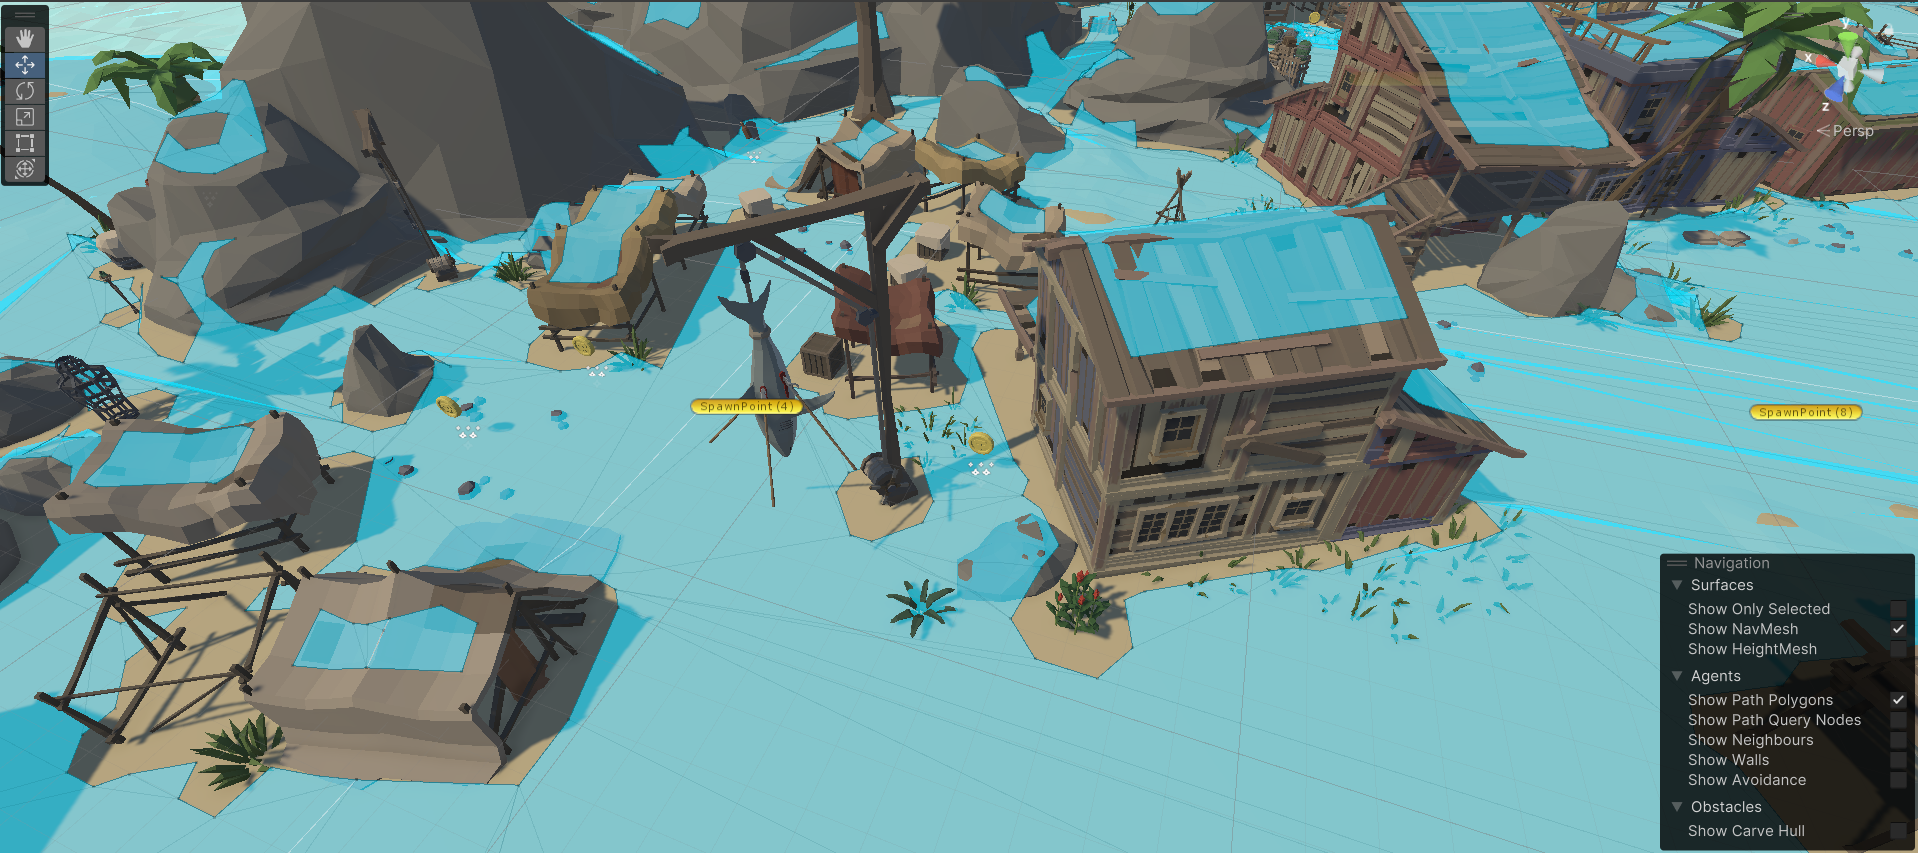
\includegraphics[width=1\textwidth]{Figures/navmesh.png}
    \caption{Vygenerovaný NavMesh pre hernú oblasť}
    \label{pic:NavMesh}
\end{figure}

Komponenta NavMeshAgent sa, ako názov napovedá, pridáva priamo na NPC agenta, kde je okrem spomínaného typu možné nastaviť aj rýchlosť, akceleráciu, či tzv. stoppingDistance, ktorá definuje, ako ďaleko pred cieľovým bodom sa agent má zastaviť. Okrem toho je možné na tejto komponente upraviť aj rôzne parametre týkajúce sa vyhýbaniu sa prekážkam. Cieľ je možné agentovi nastaviť priamo z kódu zavolaním metódy SetDestination(), ktorá sa pokúsi po vygenerovanom NavMeshi nájsť najkratšiu cestu k cieľu ak existuje.

Ďalšou komponentou špecifickou pre agenta ovládaného rozhodovacím stromom je komponenta EyeSight reprezentujúca videnie agenta. Schopnosť videnia má samozrejme aj druhý typ agenta, tá je však z dôvodov popisovaných v nasledujúcej kapitole realizovaná odlišne.

Komponenta EyeSight podobne ako komponenta Hearing implementuje generické rozhranie ISense<T> \ref{src:ISense}, tentokrát je však generikom samotný herný objekt. Nad rámec implementácie rozhrania je na tejto komponente možné nastaviť masku vrstvy hráča na ktorú reaguje príslušný RayCast a masku vrstvy prekážok, cez ktorú RayCast naopak neprejde. Taktiež je tu možné nastaviť parametre definujúce FOV ako polomer kružnice okolo agenta či uhol v rozsahu 0$^{\circ}$--360$^{\circ}$.

Narozdiel od komponenty Hearing, ktorá reaktívne odpovedá na podnety prostredia, komponenta EyeSight aktívne kontroluje prítomnosť hráčskej postavy v zornom poli. Na tento účel je vytvorená korutina EyeSightCoroutine(), ktorá je spustená v metóde Start() príslušného agenta. Túto korutinu je možné vidieť vo výpise \ref{src:EyeSightCoroutine}.

\vspace{8pt}
\begin{lstlisting}[label=src:EyeSightCoroutine,caption={Korutina zabezpečujúca videnie agenta}]
private IEnumerator EyeSightCoroutine()
{
    float delay = 0.2f;
    var wait = new WaitForSeconds(delay);

    while (isActive)
    {
        yield return wait;
        CheckEyeSight();
    }
}
private void CheckEyeSight()
{
    this.target = null;
    isActivated = false;
    this.distanceToTarget = float.MaxValue;

    Collider[] rangeChecks = Physics.OverlapSphere(transform.position, radius, targetMask);
    if (rangeChecks.Length == 0)
        return;

    Transform target = rangeChecks[0].transform;
    Vector3 directionToTarget = (target.position - transform.position).normalized;

    if (Vector3.Angle(transform.forward, directionToTarget) > angle / 2)
        return;

    float targetDistance = Vector3.Distance(transform.position, target.position);
    if (Physics.Raycast(transform.position, directionToTarget, targetDistance, obstacleMask))
        return;

    isActivated = true;
    this.target = target.gameObject;
    this.distanceToTarget = targetDistance;
}
\end{lstlisting}

Korutina teda periodicky spúšťa v definovanom intervale metódu CheckEyeSight(). Tento prístup je výhodný z hľadiska výkonu, nakoľko pri testovaní sa ukázalo, že nie je nutné aktualizovať videnie agenta pri každom vykonaní hernej slučky. 

Metóda CheckEyeSight teda získa všetky kolidery v definovanom rádiuse. Nakoľko jediný objekt obsahujúci definovanú masku vrstvy je hráčska postava, je možné priamo vziať prvý prvok v poli koliderov, ak toto pole nie je prázdne a považovať ho za hráčsku postavu. Ak by agenti boli naprogramovaní na reakcie medzi sebou, prípadne na špecifické objekty v scéne, stačilo by pridať masky týchto objektov do členskej premennej targetMask v editore, či pomocou binárnych operátorov v kóde a poľom preiterovať. Nakoľko sú ale kolidery získané v celom rozsahu kružnice, je následne získaný normalizovaný smer k hráčskej postave a overené, čí vyhovuje nastavenému kruhovému výseku. Ak je táto podmienka splnená, vykoná sa RayCast, ktorý overí, či je medzi agentom a hráčom priama viditeľnosť. Ak je splnená aj táto podmienka, je možné do rozhodovacieho procesu zaviesť informáciu, o tom, že bol spozorovaný hráč.  

\begin{figure}[!htbp]
    \centering
    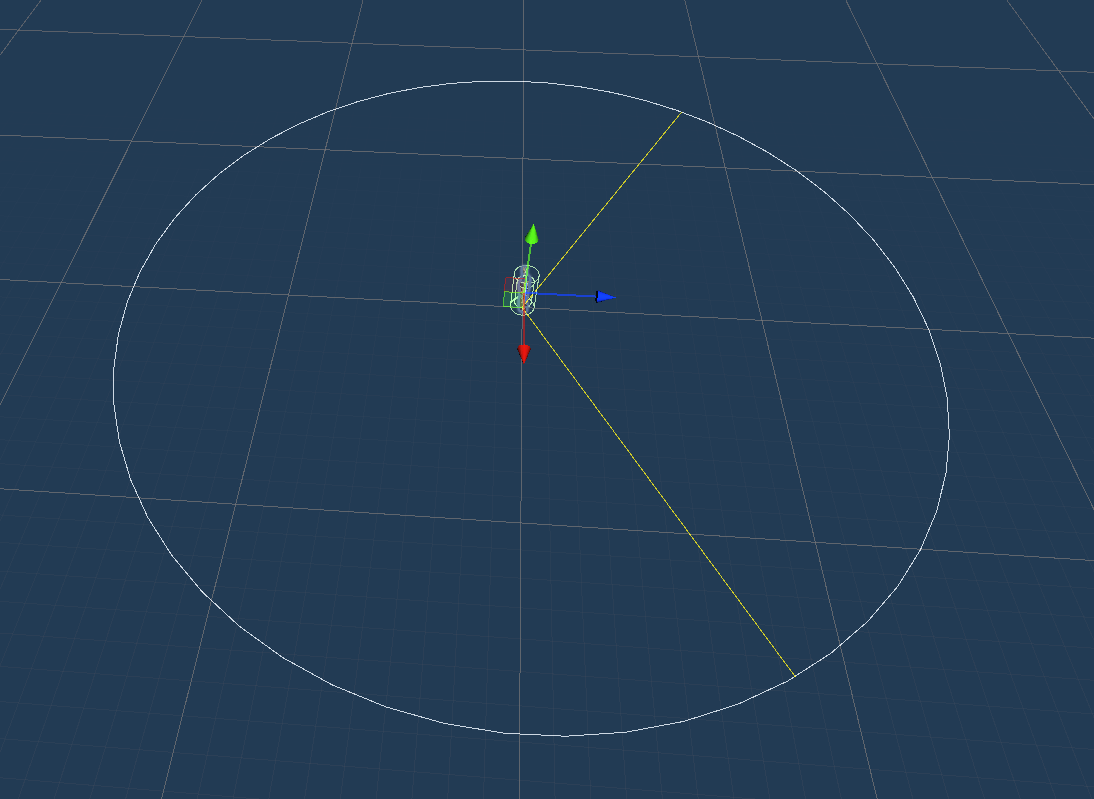
\includegraphics[width=.65\textwidth]{Figures/fov.png}
    \caption{Zorné pole NPC agenta ovládaného rozhodovacím stromom}
    \label{pic:FovDecision}
\end{figure}

Vizualizáciu zorného poľa NPC agenta využitú na ladenie je možné vidieť na obrázku \ref{pic:FovDecision}. Tá je realizovaná pomocou tzv. Custom Editoru pre triedu EyeSight, ktorý je vytvorený v Assembly-CSharp-Editor, teda osobitne od zvyšku tried, ktoré sú využívané v rámci buildu hry. V tomto editore je využitá metóda OnSceneGUI(), v ktorej je implementovaná logika vykreslovania kružnice a kruhového výseku v náhľade scény otvorenej v editore. Vizualizácia sa v reálnom čase aktualizuje v závislosti od nastavených parametrov v triede EyeSight.

\subsection{Rozhodovanie}
\label{sec:ImplDecisionTrees}
%TODO brain, state machina a vsetko okolo

\section{NPC agenti ovládaní reinforcement learningom}
\label{sec:AgentsWithBrain}
%TODO
\subsection{Prehľad špecifických komponentov}
\label{secAgentsWithBrainComponentOverview} 
% ray perceptron sensor + rigidbody + mlskeleton + behaviour params + decision requester

\subsection{Rozhodovanie}
\label{sec:ImplReinforcementLearningMLAgent}
%TODO

% Chapter 7
\chapter{Trénovanie agentov s využitím reinforcement learningu}
\label{sec:Training}
%TODO + PlayerAutomatic movement, scriptedPath, waypointy, navmesh - len ze uz bol vysvetleny
\section{Prvý trénovací scenár}
\label{sec:FirstScenario}
%TODO
%... 
\section{N-tý trénovací scenár}
\label{sec:LastScenario}
%TODO

% Chapter 8
\chapter{Porovnanie prístupov}
\label{sec:ImplReinforcement learning}
%TODO
\section{Porovnanie z hľadiska výkonu}
\label{sec:Performance}
%TODO
\section{Empirické porovnanie}
\label{sec:Gameplay}
%TODO

% Chapter 9
\chapter{Záver}
\label{sec:Conclusion}

%Template/Testing
\begin{figure}[!htbp]
	\centering
	
\includegraphics[width=.5\textwidth]{Figures/FEI_CZ.pdf}
	\caption{Test}
	\label{pic:Teeest}
\end{figure}

\begin{center}
\begin{tabular}{ c c c }
 cell1 & cell2 & cell3 \\ 
 cell4 & cell5 & cell6 \\  
 cell7 & cell8 & cell9    
\end{tabular}
\end{center}

\begin{lstlisting}[label=src:Test,caption={Test}]
// Hello World! program
namespace HelloWorld
{
    class Hello {         
        static void Main(string[] args)
        {
            System.Console.WriteLine("Hello World!");
        }
    }
}
\end{lstlisting}
%End of Template/Testing

% Prílohy
%\appendix
%\input{appendix_mono}

\printbibliography[title={Literatúra}, heading=bibintoc]
\end{document}
